\chapter{Experimental Apparatus}

\section{CERN Laboratories}

\subsection{Funding Model}

The CERN operating budget provided by the individual member states. The size of the contribution is determined:
\begin{quote}
``using the arithmetic average of three years of Net National
Income values until year before last year and applying the corresponding annual average
exchange rate for each year''
\end{quote}
Here the Net National Income is defined as:

\begin{center}
\begin{table}[]
\begin{center}
\caption{A summary of the GDP, CERN lab contribution, and the ratio between GDP and the absolute contribution 
by country}
\begin{tabular}{cccc}
\textbf{Country} & GDP & Abs (Rel) Cont. & (Cont/GDP) $\times 10^{-7}$ \\
\hline
Germany & \$3.36T  & 231M CHF (20.5\%) & 6.8 CHF/USD  \\
France  & \$2.24T  & 170M CHF (15.1\%) & 7.5 CHF/USD\\
UK      & \$2.86T  & 161M CHF (14.3\%) & 5.6 CHF/USD\\
Italy   & \$1.82T  & 125M CHF (11.1\%) & 6.9 CHF/USD\\
Spain   & \$1.19T  & 88M  CHF (7.82\%) & 7.4 CHF/USD\\
\hline
USA     & \$18.03T & -             & -     \\
\end{tabular}
\end{center}
\label{tab:gdpcontrib}
\end{table}
\end{center}

\begin{center}
\begin{table}[]
\begin{center}
\caption{CMS Gender Demographics by Age as of 2014. Age groups are separated by age range. Each column sums to 100\% of the given gender.
There are a total of4119 Males and 863 females. This corresponds to a global gender ratio of 4.77 men to every 1 female. The ratio is 
between the absolute numbers of men and women within that age range.}
\begin{tabular}{cccc}
\textbf{Age Range} & \textbf{\% of Men} & \textbf{\% of Women} & \textbf{Male/Female Ratio}\\
\hline
$<$ 25 & 12.6\% & 19.4\% & 3.1  \\
25-29 & 20.0\% & 24.0\% & 4.0  \\
30-34 & 12.8\% & 15.0\% & 4.2  \\
35-39 & 9.7 \% & 8.4\%  & 5.0  \\
40-44 & 8.5\%  & 8.3 \% & 4.9  \\
45-49 & 8.3\%  & 7.2 \% & 5.5  \\
50-54 & 8.5\%  & 7.0\%  & 5.8  \\
55-59 & 6.6\%  & 5.0\%  & 6.3  \\
60-64 & 5.2\%  & 2.6\%  & 9.8  \\ 
65-69 & 3.8\%  & 2.1\%  & 8.7  \\
$>$69  & 4.1\%  & 0.6\%  & 34 \\ 
\end{tabular}
\end{center}
\end{table}
\end{center}
 
\begin{center}
\begin{table}[]
\begin{center}
\caption{Differences in Aboslute NNI vs GDP for the year 2015. Countries are ordered by absolute 
contribution size from highest to lowest.}
\begin{tabular}{ccccc}
\textbf{Country} & \textbf{GDP [USD]} & \textbf{NNI [USD]} &  \textbf{NNI/GDP} & \textbf{NNI/Capita}    \\
\hline
Germany & 3.36T & 3.31T & 0.99 & 40.6k\\
France  & 2.24T & 2.27T & 1.01 & 34.4k\\
UK      & 2.86T & 2.33T & 0.81 & 35.8k\\
Italy   & 1.82T & 1.84T & 1.01 & 30.3k\\
Spain   & 1.19T & 1.33T & 1.12 & 28.6k\\
\hline
USA     & 18.03T & 15.67 & 0.87 & 48.7k\\
\end{tabular}
\end{center}
\label{tab:nnicontrib}
\end{table}
\end{center}


\begin{figure}
\begin{center}
%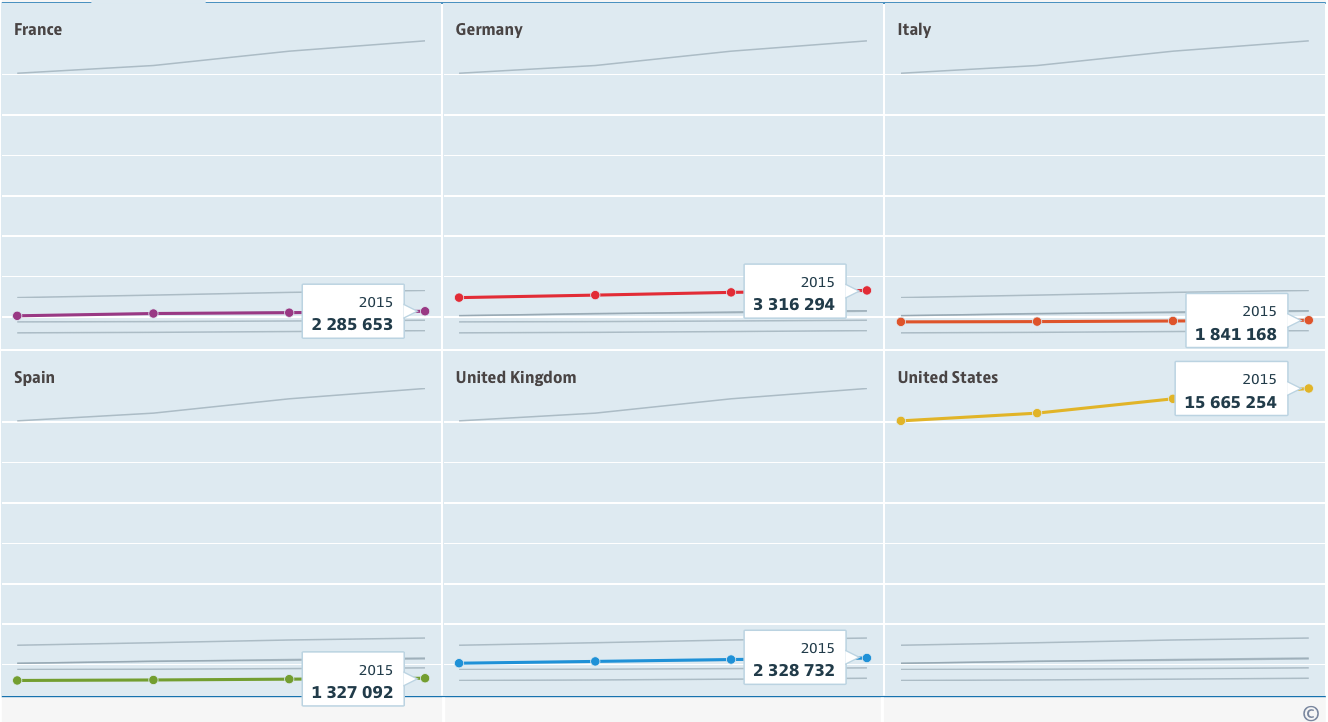
\includegraphics[width=.95\textwidth]{pics/NNI}
\caption{Net National Income for member countries over the three year period used in the average 
generating the 2015 budget for CERN Laboratories}
\end{center}
\end{figure}

\subsection{Organizatiional Structure}



\section{The Large Hadron Collider}

\begin{figure}
\begin{center}
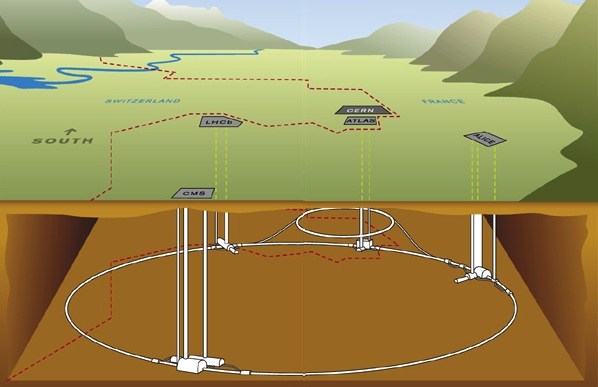
\includegraphics[width=.7\textwidth]{lhc_tunnel}
\caption{The LHC tunnel installed on the border of Geneva, Switzerland and France. 
The experiments are distributed along the circumference of the ring.}
\end{center}
\end{figure}

\begin{figure}
\begin{center}
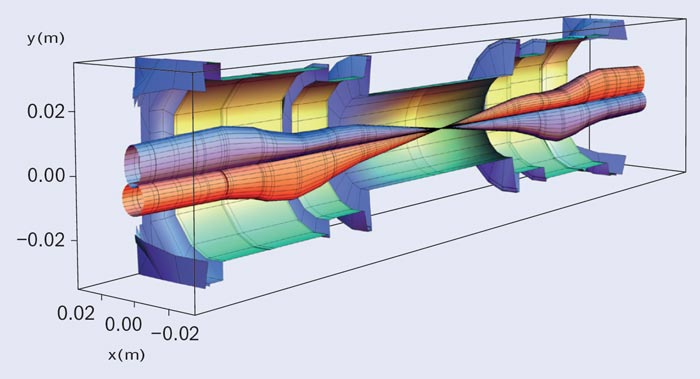
\includegraphics[width=.7\textwidth]{pics/beam_squeeze}
\caption{Squeeze}
\end{center}
\end{figure}


\begin{center}
\begin{table}[]
\begin{center}
\caption{LHC Running Parameters \cite{lhcparams}}
\begin{tabular}{ccc}
\textbf{Parameter} & \textbf{Value} & \textbf{Remarks} \\
\hline
Circumference (km) & 26.7 km & 100-150 m underground\\
Number of Dipoles & 1232 & Nb-Ti Cables \\
Length of Dipole & 13.3 m & \\
Dipole Field Strength & 8.4 T & Results form high beam energy \\
Operating Temperature & 1.9 K & He cooled superconducting magnets\\
Current in Dipole Coils & 13kA & Results from high magnetic field \\
Beam Intensity & 0.5 A & \\ 
Beam Stored Energy & 362 MJ & 1MJ melts 2kg Cu \\
Magnet Stored Energy / octant & 1100 MJ & \\
\end{tabular}
\end{center}
\end{table}
\end{center}


The bunches of protons in the LHC are bent into a circular trajectory by more than 1200
 superconducting dipole magnets and are focused and maintained close to the ideal
 orbit around the ring by hundreds of superconducting quadrupole magnets. 
Thousands of corrector magnets around the ring allow the beam to be steered closer 
to the ideal orbit, make the focusing independent of the particles’ energy variations
 within a bunch, and cancel the effects of higher order multipoles in the fields induced 
by small field imperfections in the main magnets. 
The radiofrequency (RF) field in superconducting cavities is placed periodically around 
the ring and accelerates the protons from the injection energy of 450 GeV to the final
 operating energy, which is designed to be 7 TeV per beam. The RF field also causes the
 protons to be bunched, as only particles at or near a certain ”equilibrium phase” on 
the RF wave will be accelerated stably. Special quadrupoles around each interaction region
 focus the bunches down to a small transverse size, to increase the likelihood of a
 proton-proton collision each time two bunches pass through each other.


\textbf{Source of Pile Up Interactions}

pile up events per event cross is the total inelastic cross section times the luminosity divided by the bunch collsion rate. This is respectively $8.5\times 10^{-26}\text{cm}^2 \times 10^{34}\text{cm}^{-2}\text{s}^{-1}/ (32 \times 10^6 \text{s}^-1 \approx 27$ (cite:arXiv:1204.5689). 

\section{Other LHC Related Experiments}

\section{Compact Muon Solenoid Experiment (CMS)}

Physics from a theoretical point of view can consider particles in terms of their kinematic 
phase space, however, on cannot make direct measurements of the hard scattering process. Instead,
detectors are built to indirectly measure the energy and momenta of the final state particles.
To do this, a layered system of sub detectors is used to perform particle identification. By relying on known interactions of standard model particles with detector materials 
strong probabilitistic statements can be made the flavor of particles in a given collision. 
By building a heremetic detector and integrating the various subdetectors in a given 
solid angle, one obtains a wholeistic view of the fundamental physics.
This section will discuss each subdetector, the particles it is used to identify, and the 
underlying physics which allows the individual measurements to be made.


\begin{figure}
\begin{center}
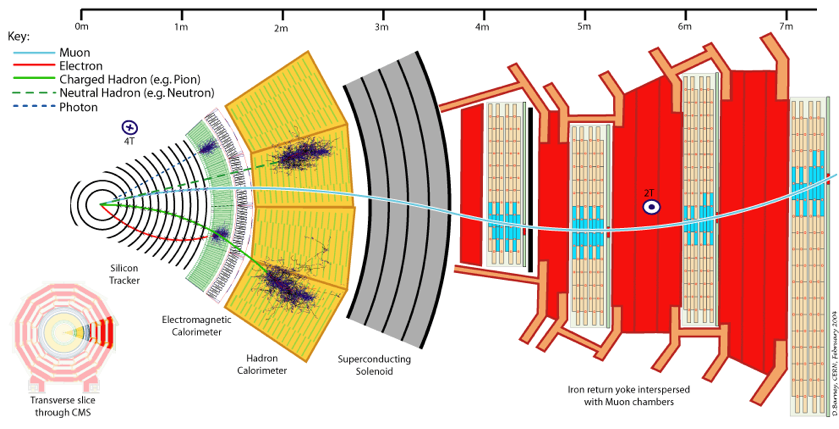
\includegraphics[width=.95\textwidth]{pics/cms_transverse}
\end{center}
\caption{ A tear-away view of the inner detectors of CMS.}
\label{fig:cms_transverse}
\end{figure}

\begin{figure}
\begin{center}
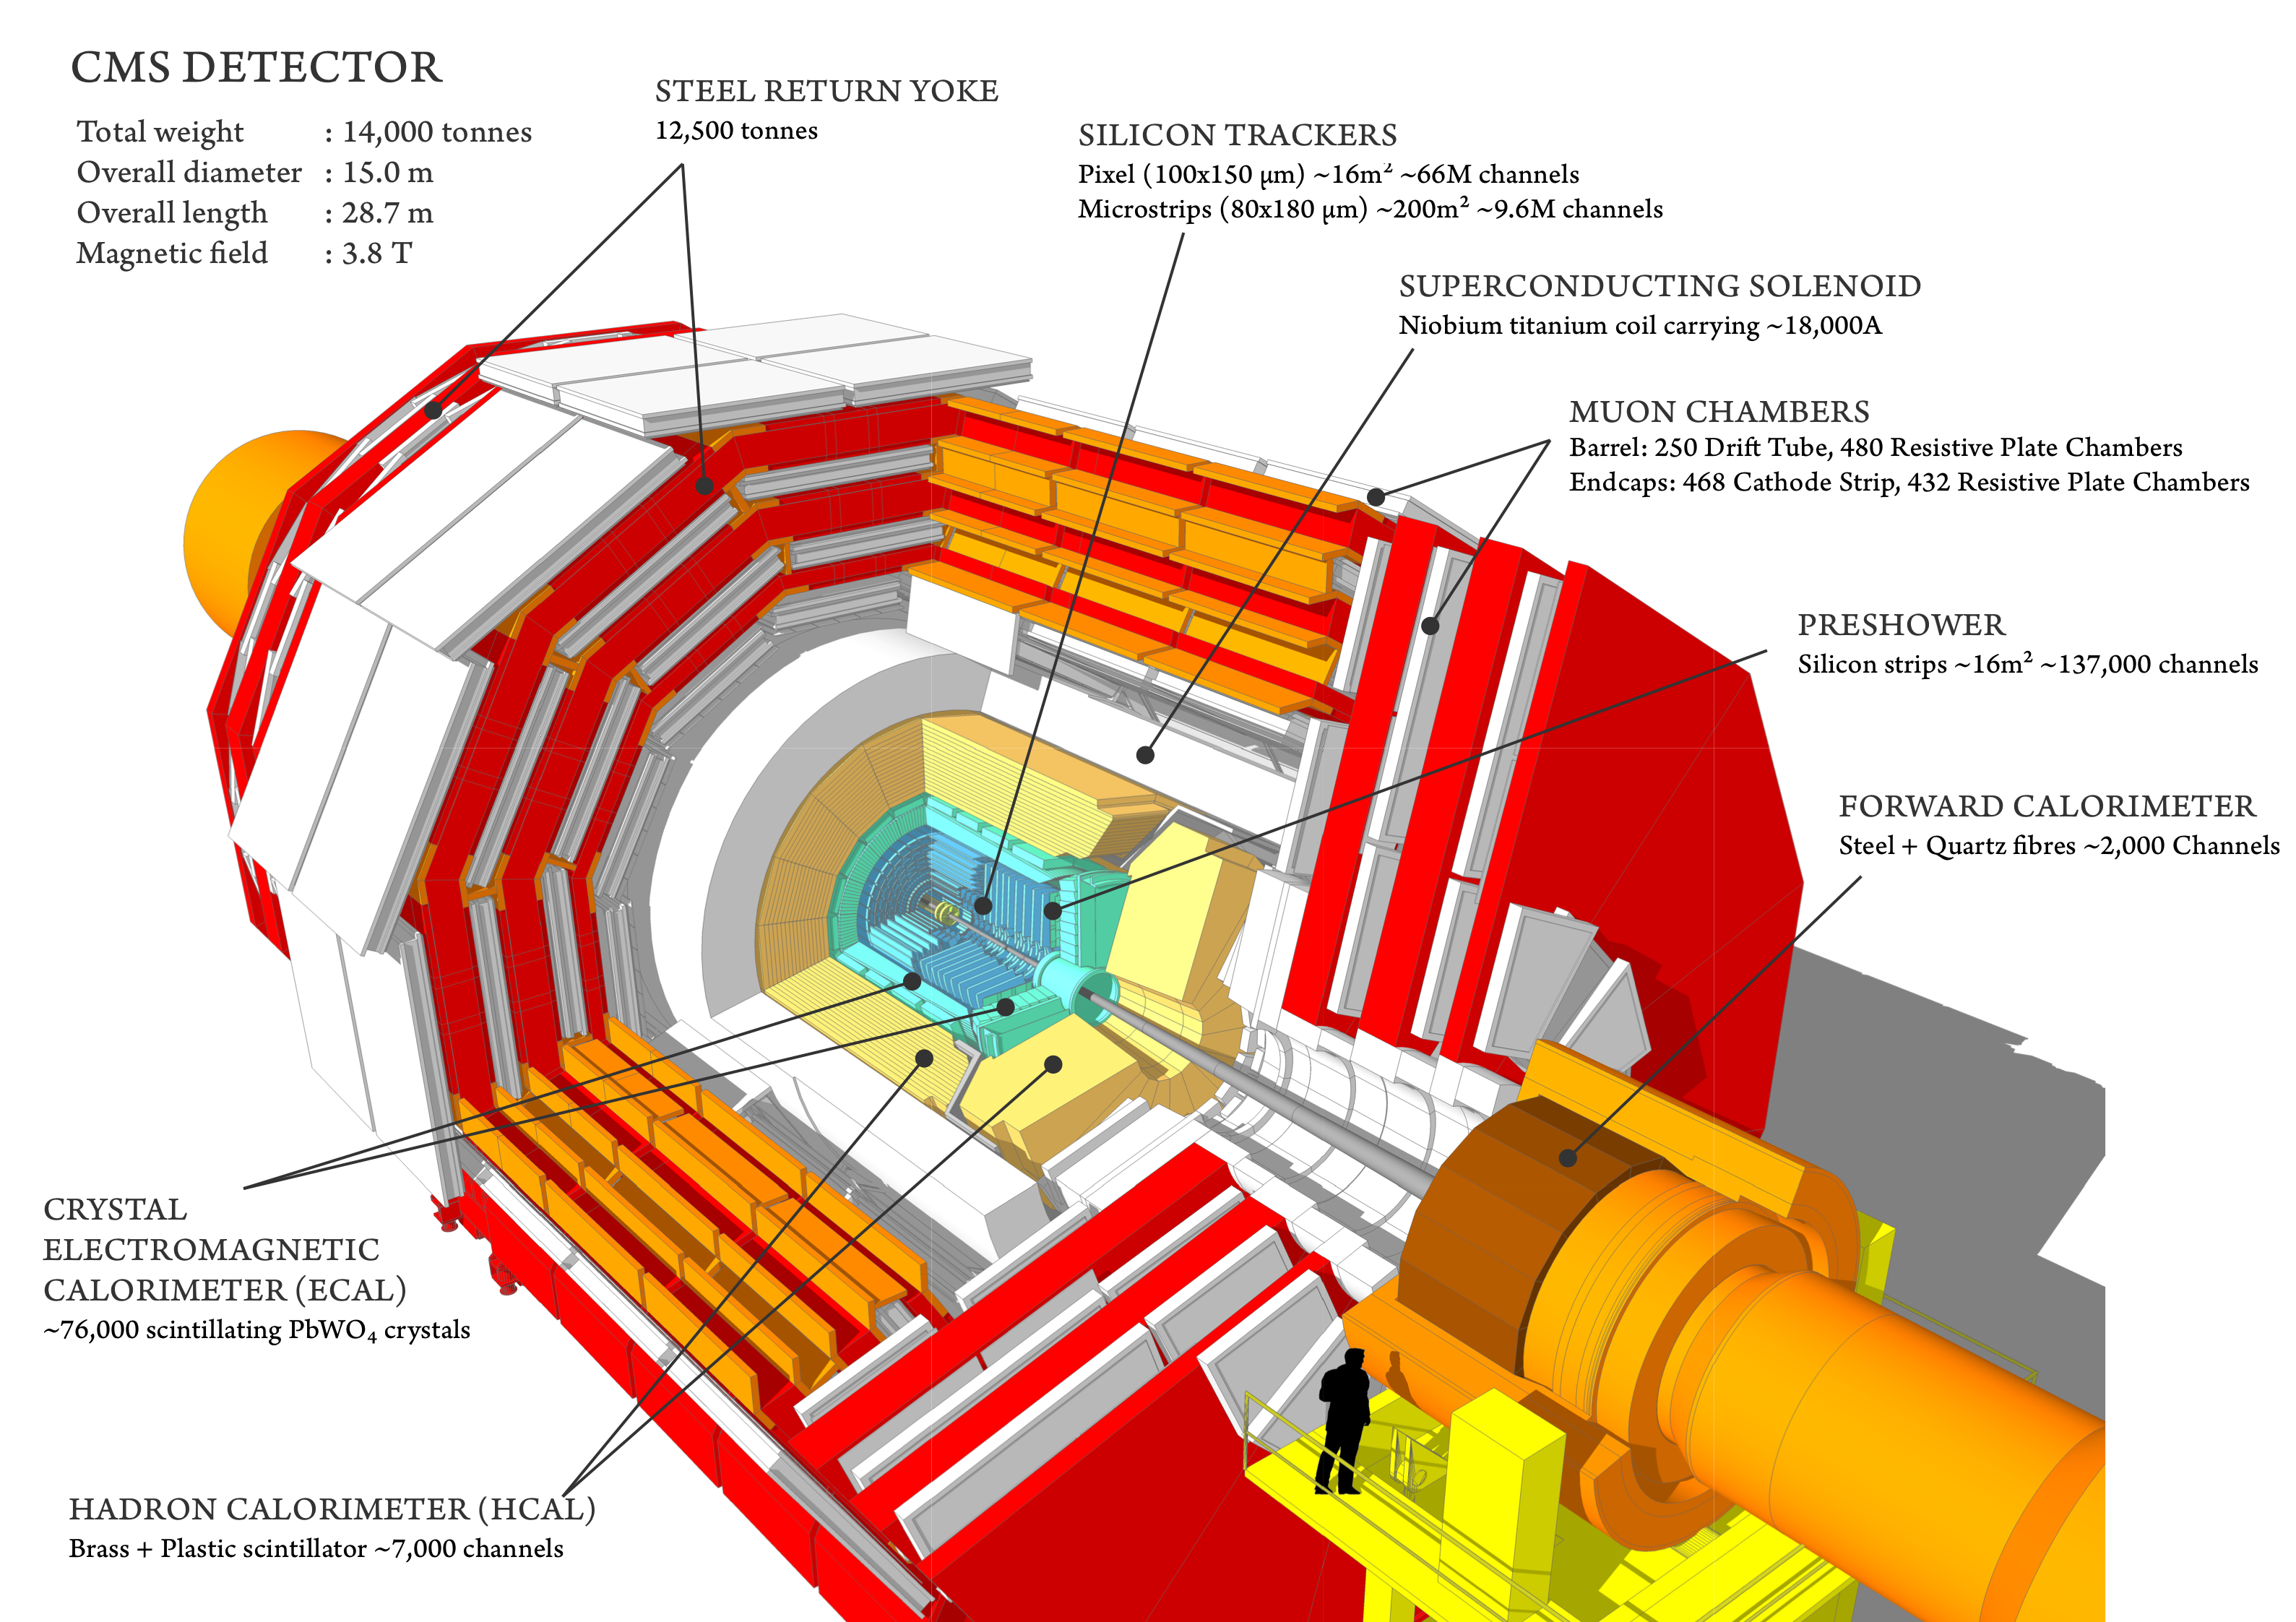
\includegraphics[width=.90\textwidth]{pics/cut_away_view}
\end{center}
\caption{Cut away view of the CMS Detector}
\label{fig:cms_onion}
\end{figure}

The Compact Muon Solenoid (CMS) Detector is a general-purpose detector consisting of 
an all silicon tracker, a precision electromagnetic calorimeter (ECAL), a hadron calorimeter
 (HCAL), a 4 T superconducting solenoid and muon chambers. The solenoid deflects charged
 particles whose paths are traced in the tracker, making it possible to 
reconstruct the particles’ momentum. The two calorimeters reconstruct the energy 
of and identify photons, electrons and hadronic jets.
As shown in Figure \ref{fig:cms} the detector has cylindrical symmetry about the
 interaction point where the proton beams collide. By maintaining near full coverage 
of the interaction point it is possible to detect signatures such as neutrinos or other weakly interacting particles as missing energy. 

\subsection{Electromagnetic Calorimeter (ECAL)}


\begin{figure}
\begin{center}
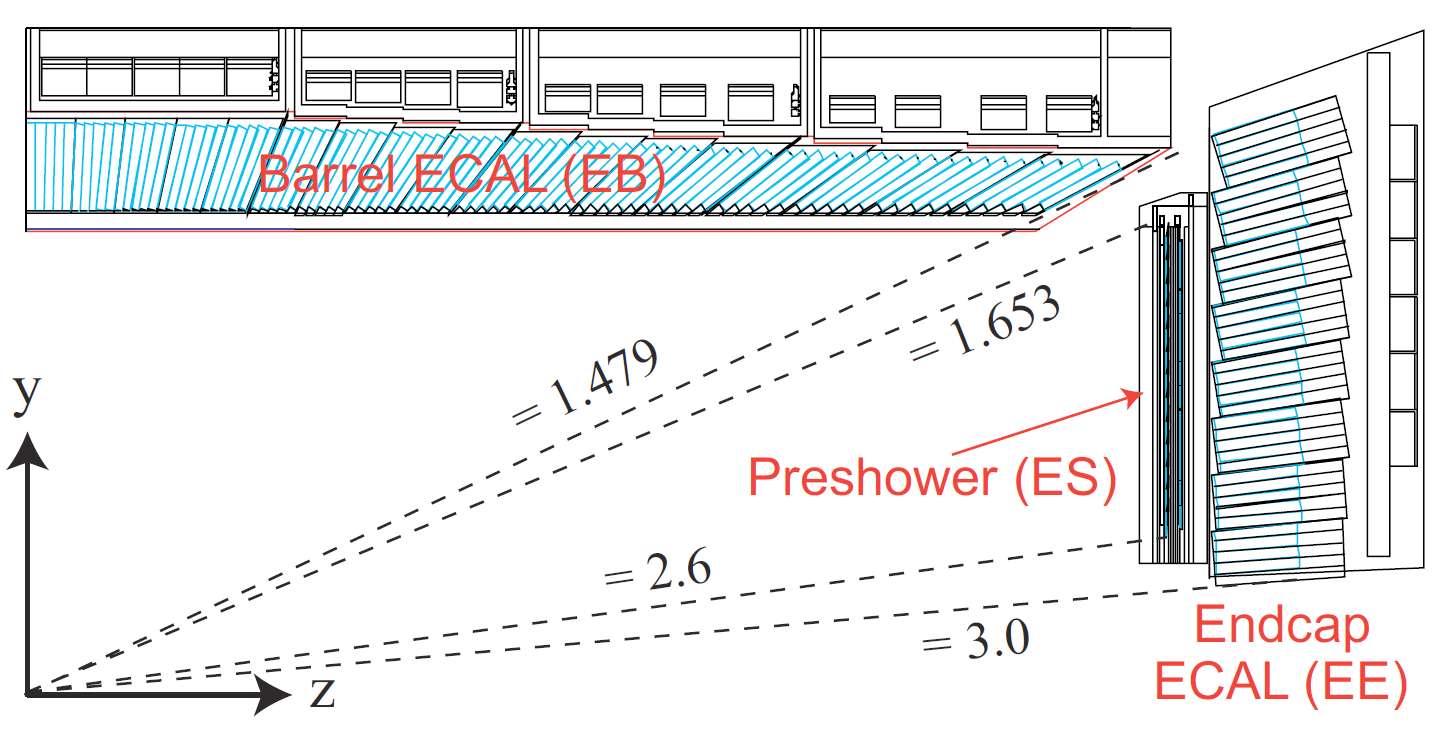
\includegraphics[width=.95\textwidth]{pics/ecal_diagram_side}
\end{center}
\caption{Kinematic coverage of the electromagnetic calorimeter (ECAL) barrel and endcap}
\label{fig:ecal}
\end{figure}

The electromagnetic calroimeter (ECAL) exists to measure the energy of eletromagnetic
showers of electrons and photons.  

For high energy electromagnetic objects, that is above the mass threshold of 
pair production: $\gamma \rightarrow e^+e^-$, the interaction with matter occurs as an electromagnetic shower. In this shower, photons pair produce electron-positon pairs and
 electrons undergo bremmstrahlung 
radiation: $e^\pm \rightarrow \gamma e^\pm$. This processes continues until 
the individual particles in the shower cannot continue $1\rightarrow 2$
 processes and instead undergo multiplicity presverving iteractions such 
as compton scattering and ionization.

The detector material (for CMS a scintillating crystal) is characterised the shower's
 Moliere Radius, defined as the radius
 (transverse to the incidence) of a cylinder that contains 90\% of the shower. For the CMS ECAL, 
crystals are of approximately the Moliere radius 2.2 cm. The material can further
be characterized by it's radiation length, the typical amount of matter the incidient particle
can traverse before an interaction. The CMS crystals have a relatively short radiation
 length of 0.9 cm. Each crystal is approximately 25 radiation lengths = 23 cm. 

The cystal energy resolution as a function of energy is characterised as:
\begin{equation}
\frac{\sigma(E)}{E} = \frac{S}{\sqrt{E}} \oplus \frac{N}{E} \oplus C
\end{equation}
Here $\sigma$ is the gaussian standard deviation of the energy measurement, the operator $\oplus$ signifies addition in quadrature, $S$ the stochastic term, $N$ the
electronic readout noise, and $C$ the constant term which does not scale with energy. The 
stochastic term $S$ comes from the staistical nature of the photoelectric shower and the 
containment within the crystal. The readout term arises from the electronics noise in the preamplifier and digitization of the signal. The constant term $C$ is caused by non uniformities between
the many crystals and is ultimately dominated by the crystal to crystal intercalibration. As
the first two term scale inversely with energy the constant term for high energy photons and electrons $> 50$ GeV is dominant. The design energy resolution for high energy photons like those
found in the discovery of the Higgs bosom is $< 0.5\%$

\begin{figure}
\begin{center}
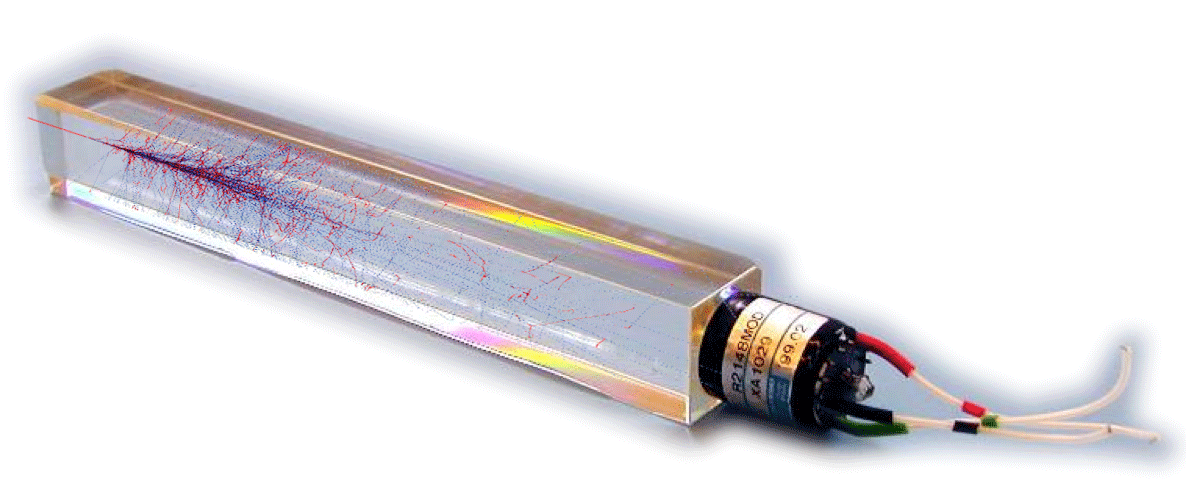
\includegraphics[width=.45\textwidth]{pics/ecal_crystal}
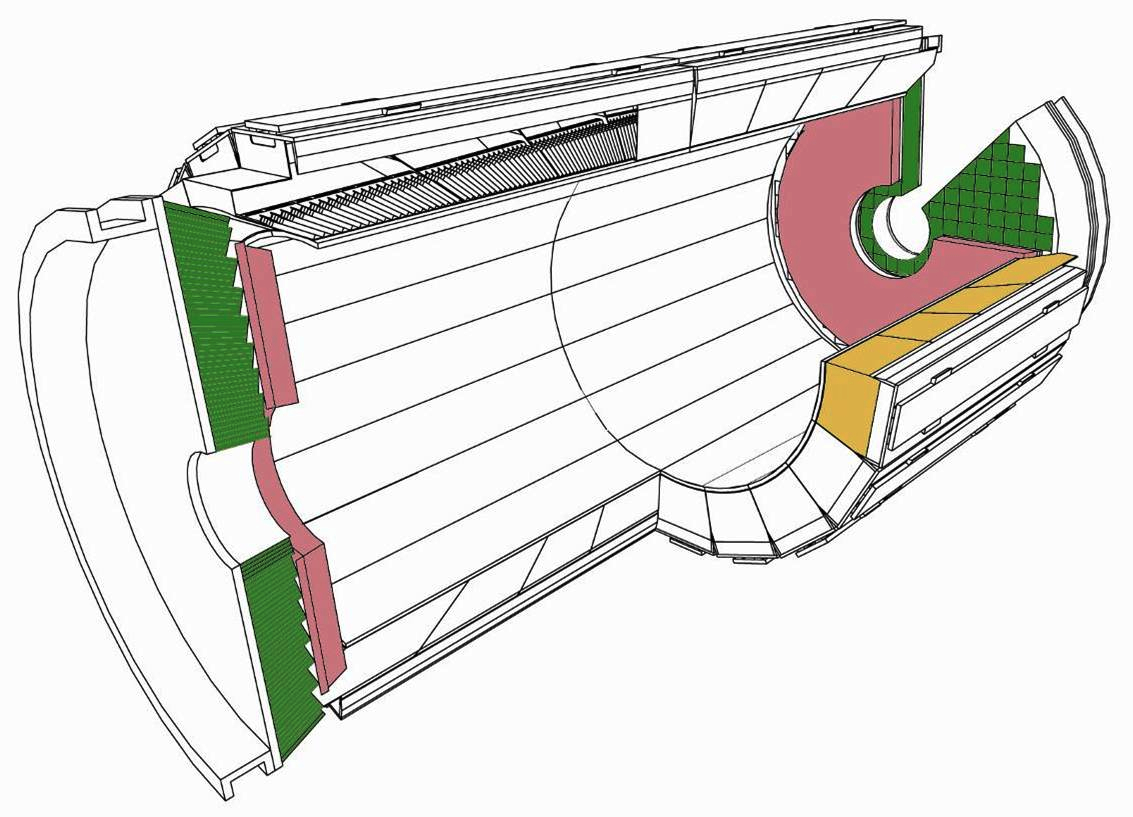
\includegraphics[width=.45\textwidth]{pics/ecal_diagram}
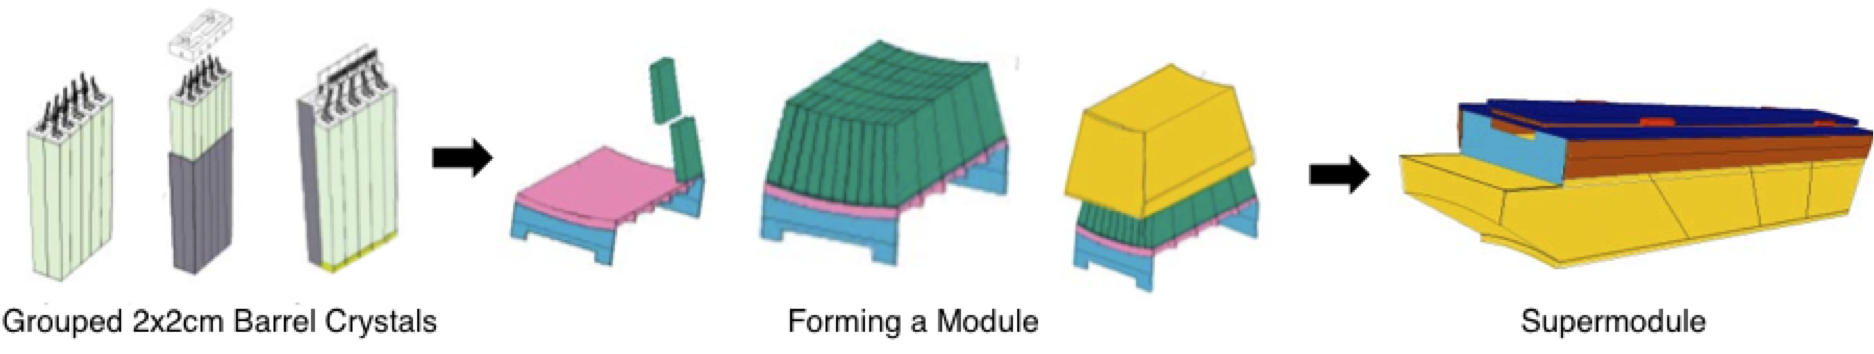
\includegraphics[width=.95\textwidth]{pics/Supermodule}
\end{center}
\caption{A single CMS ECAL Crystal (top left) tearaway view of distribution of crystals (top right) The construction of a single supermodule (bottom)   }
\label{fig:ecal_cryastal}
\end{figure}

\begin{figure}
\begin{center}
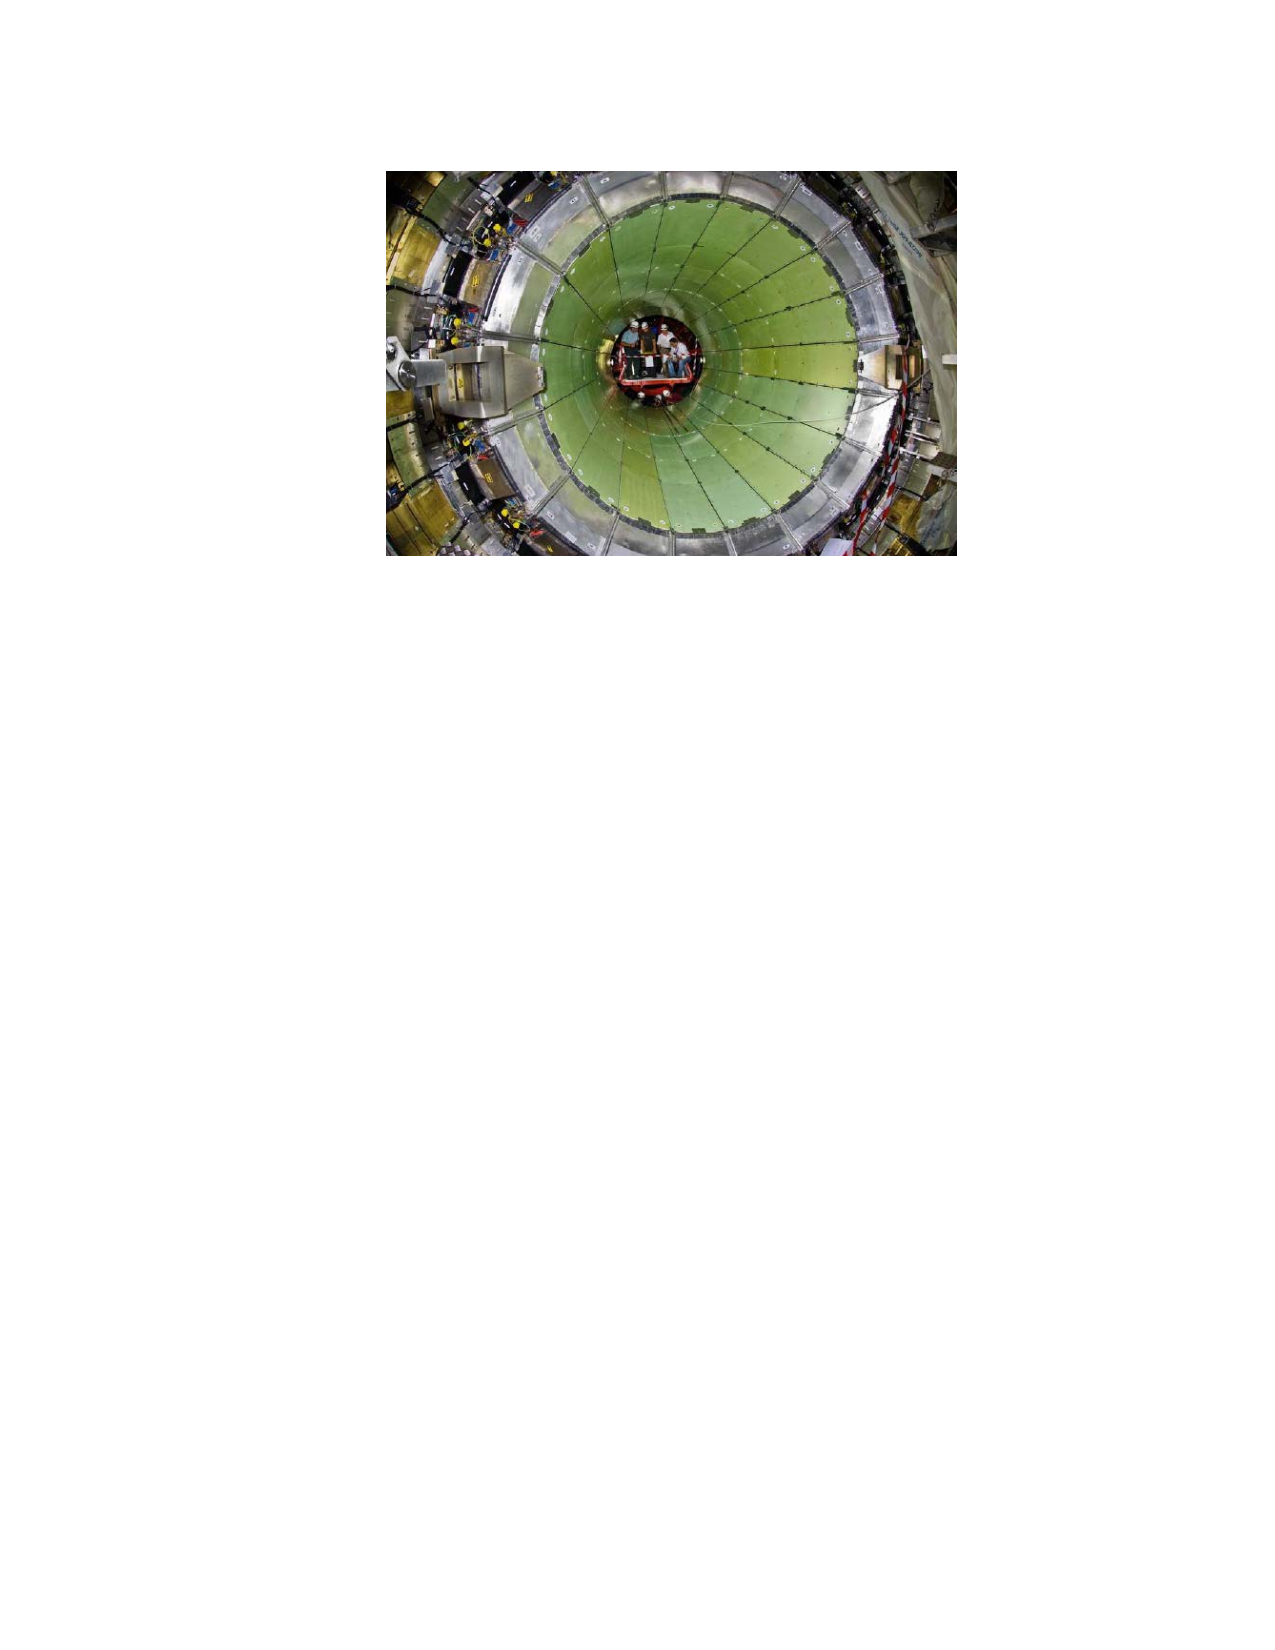
\includegraphics[width=.45\textwidth]{pics/ecal_barrel}
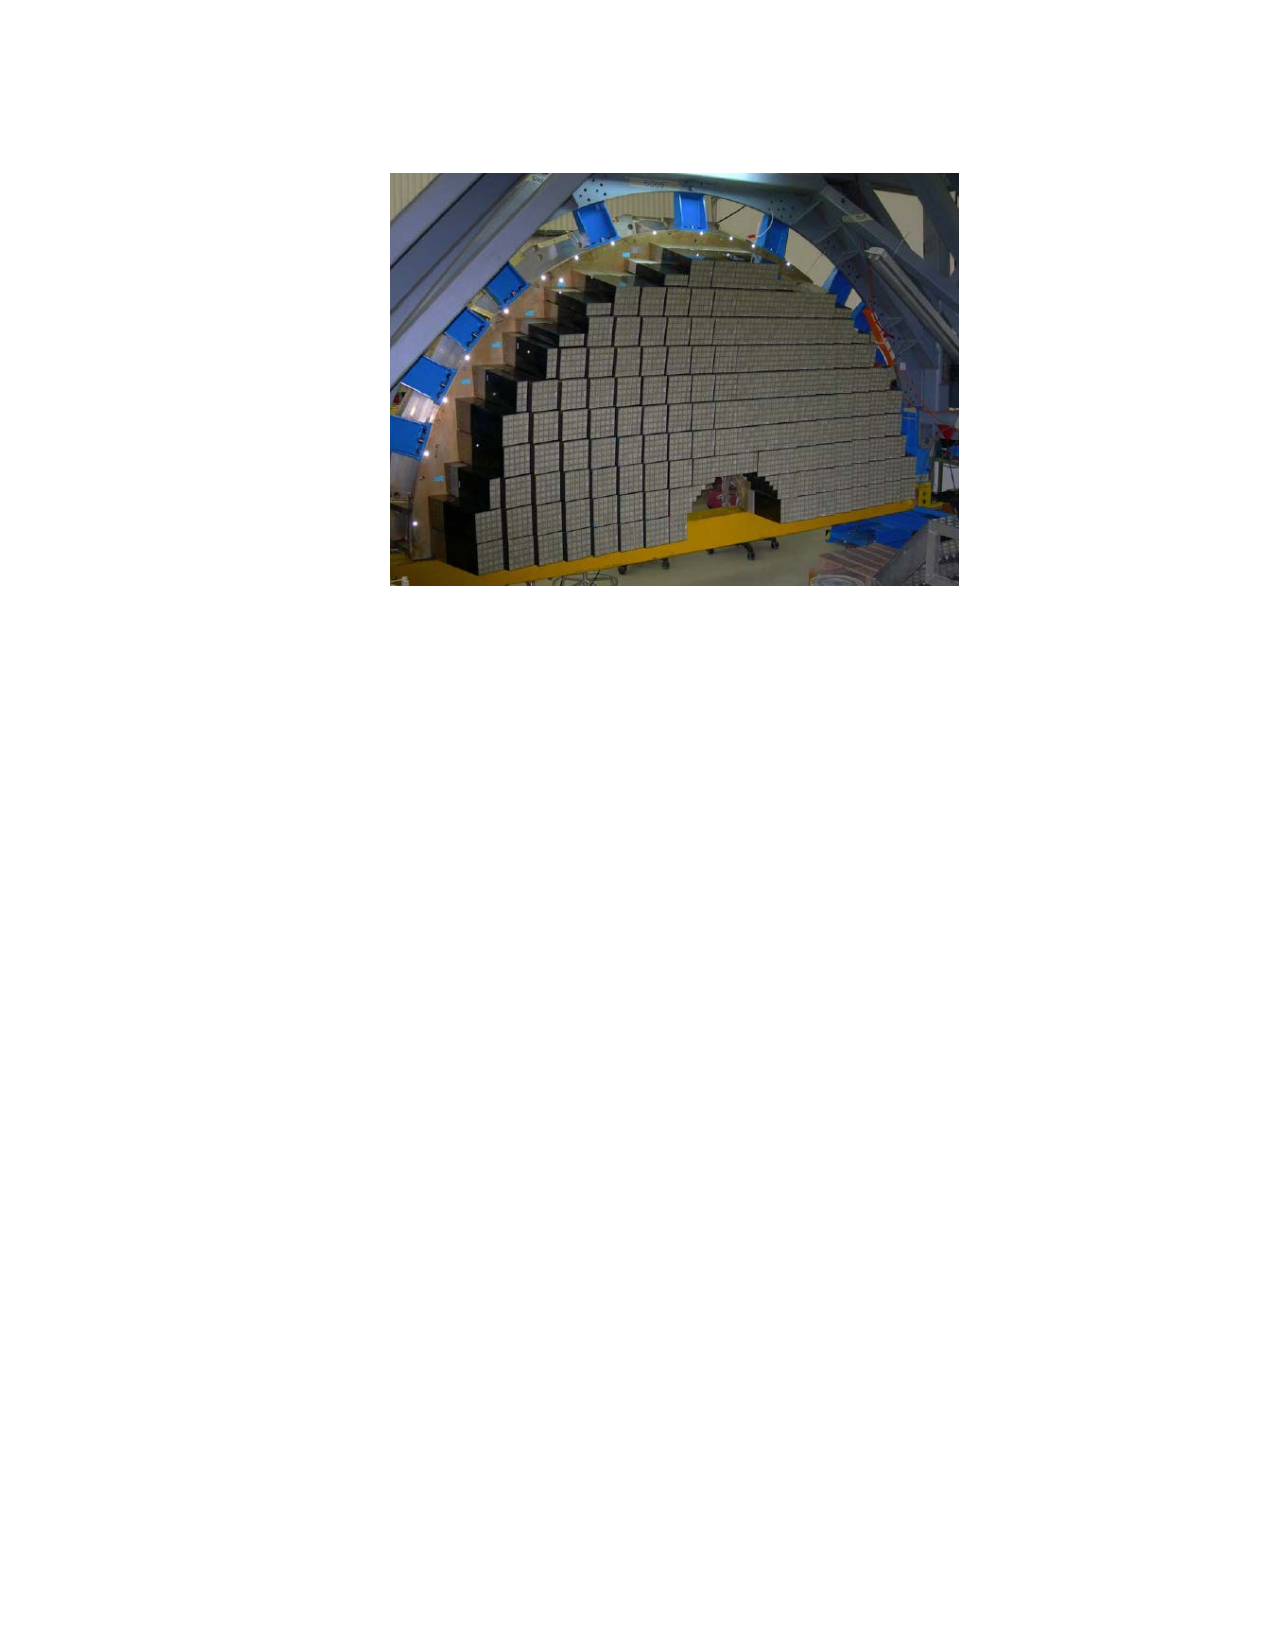
\includegraphics[width=.45\textwidth]{pics/ecal_dee}
\end{center}
\caption{The ECAL barrel installed within CMS (left) A single Dee of the ECAL endcap (right)}
\label{fig:ecal_photos}
\end{figure}

The ECAL consists of 75,848 Lead Tungstate PbWO$_4$ scintillating crystals Fig. \ref{fig:ecal_crystal}. The ECAL is separated into two sections: the Endcaps and the Barrel. 
The Barrel consists of 61200 2x2x23 cm$^3$ crystals separated into 36 Supermodules  and is contained in $|\eta| < 1.48$. The Endcaps are separated into 4 Dees (Fig. \ref{fig:ecal_photos})
 of 3662 crystals with each crystal measuring 3x3x22 cm. 
The 4 dees cover a  pseudorapidity range between $1.48 < |\eta| < 3.0$.
The Endcaps are behind a preshower detector, composed of two lead absorbers 
interleaved with silicon detectors. The preshower covers the pseudorapditiy range
of $1.653 < |\eta| < 2.6$ with each silicon sensor covering a square are of 
63 mm x 63 mm divided into 32 strips. The preshower is designed to give significantly
better spatial resolution than using the endcap alone to aid in the separating single photons
and $\pi^0 \rightarrow \gamma\gamma$ decays used to calibrate the endcap. As the first layer is
2 radiation wavelengths thick such that the majoirty of incident single photons will  
begin to shower before reaching the second layer.  


The preshower converts many of the photons, 
which assists in distinguishing directly produced photons from pairs
of photons resulting from neutral pion decays. 

The light in each crystal is collected as a current 
and amplified by avalanche photodiodes (APDs) in the barrel
region and vaccuum phototriodes (VPTs) in the endcap. This transition is
necessary as the endcap region must be tolerant to much
higher levels of radiation damage from softly scattered (low momentum transfer $Q^2$)
interactions. 

\begin{figure}
\begin{center}
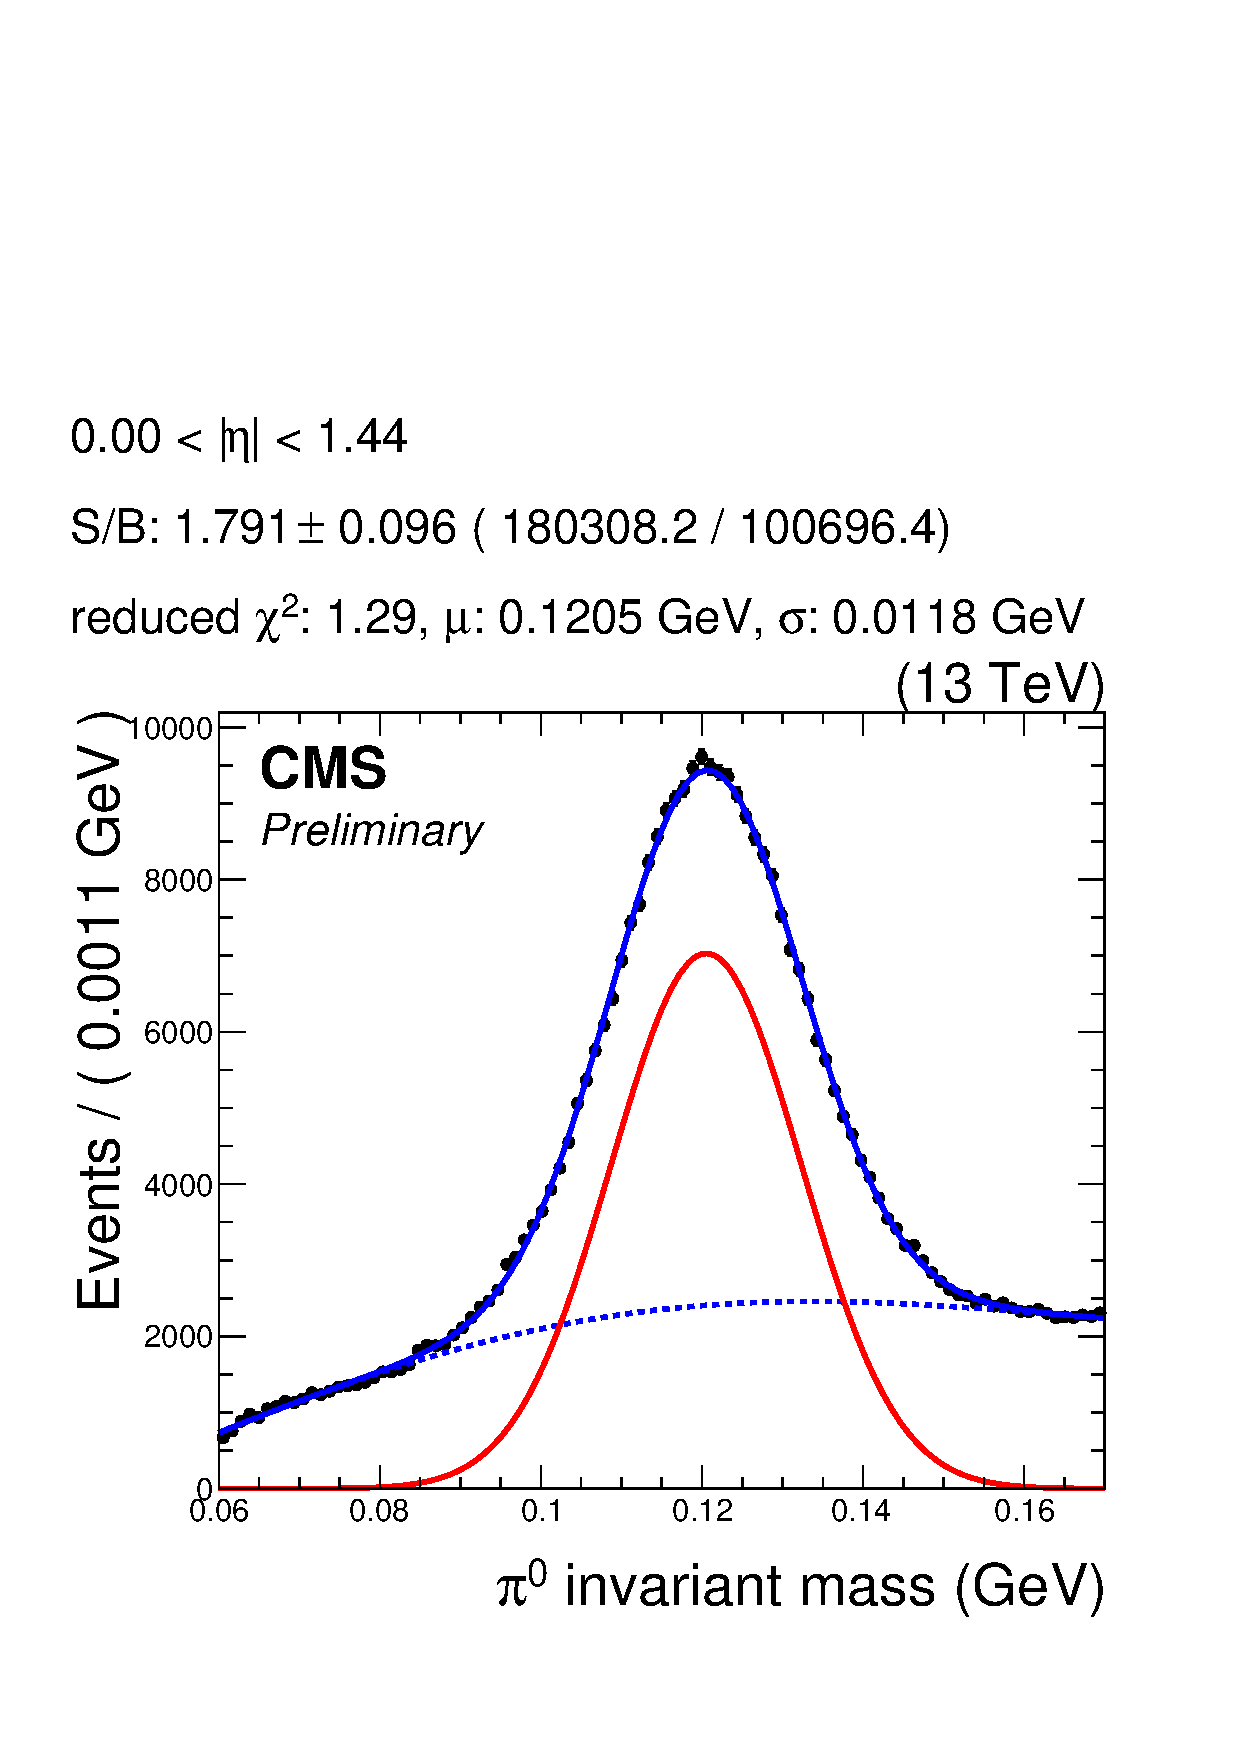
\includegraphics[width=.45\textwidth]{pics/pizero_eb}
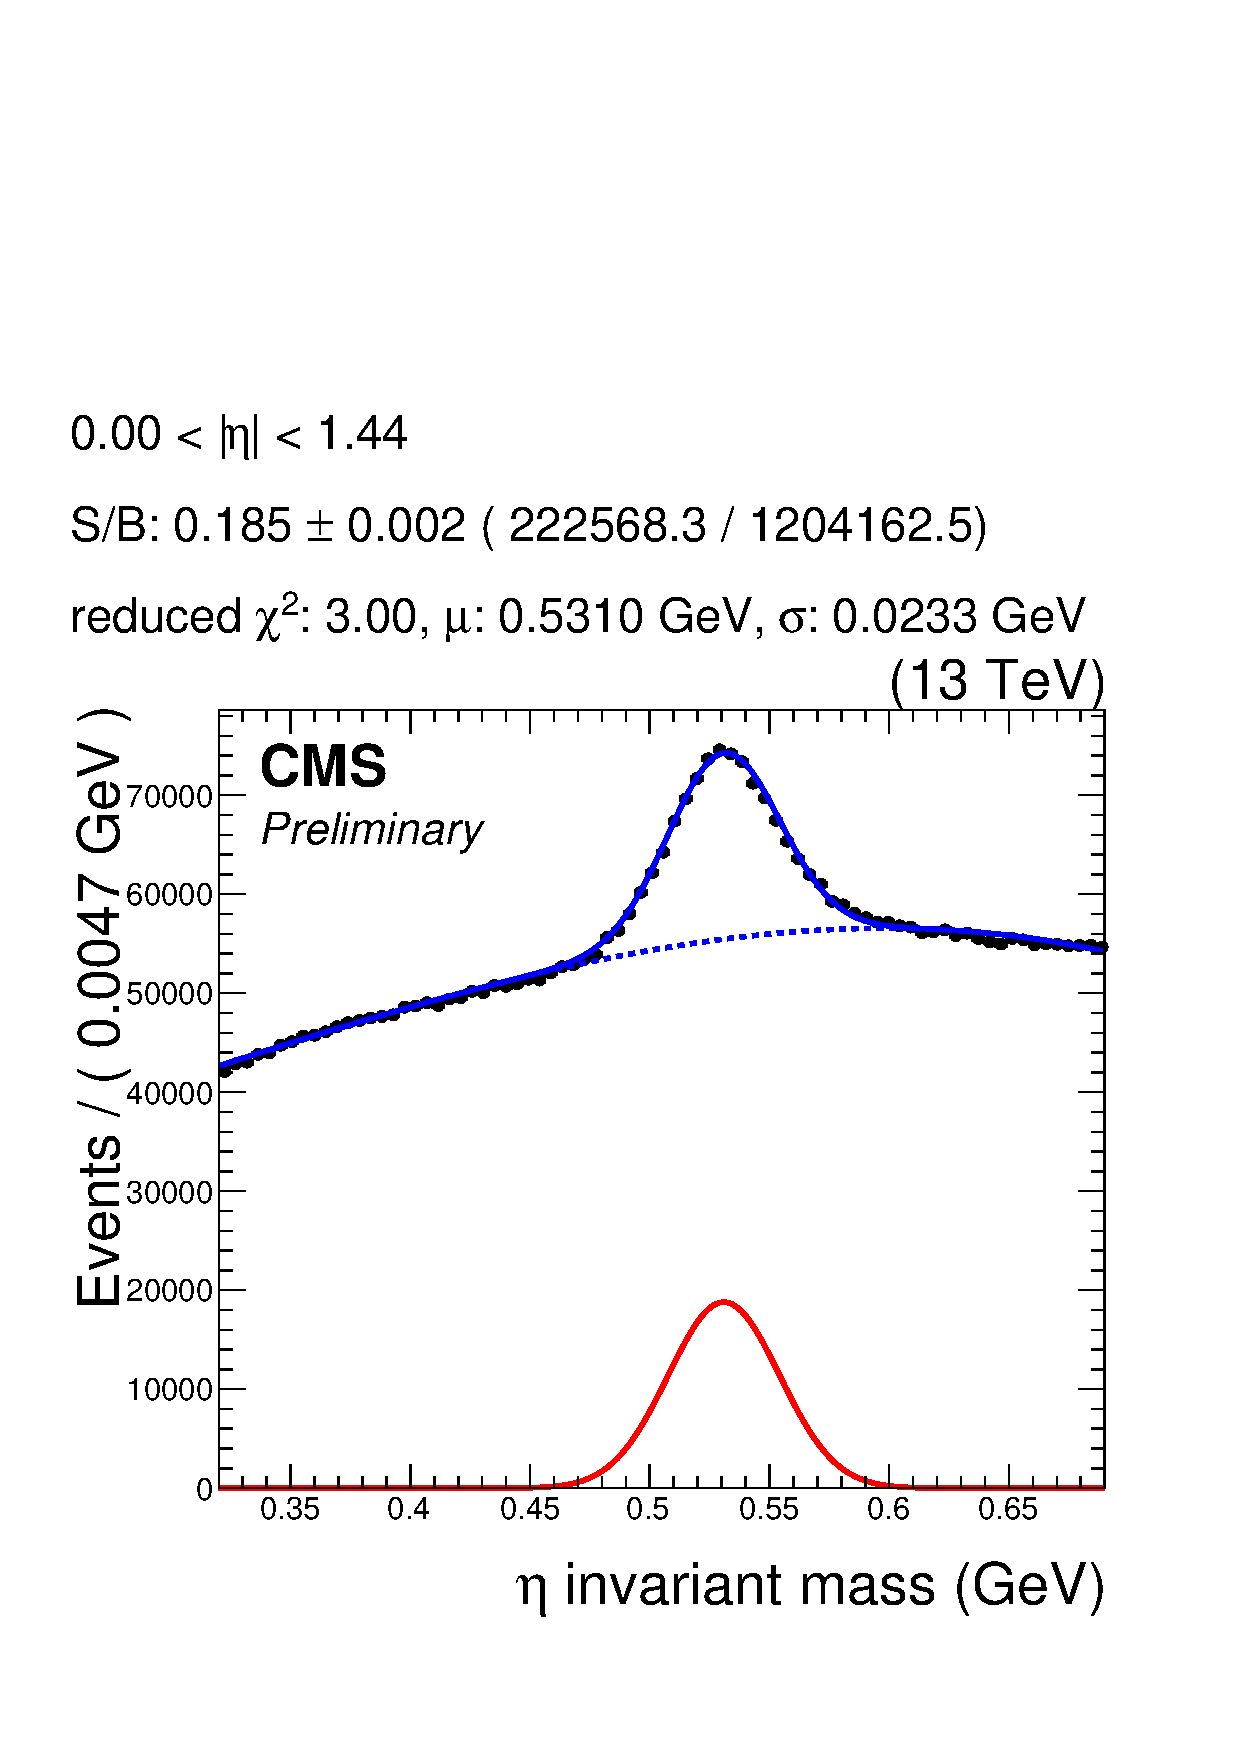
\includegraphics[width=.45\textwidth]{pics/eta_eb_2015b}
\end{center}
\caption{Calibration stream outputs for the pizero and eta barrel trigger paths}
\label{fig:pizero_eta}
\end{figure}

The detector is calibrated with a method that reconstructs the mass of neutral
pion and eta-mesons to precisely calibrate the entire ECAL. The copious
production of these particles in hadronic jets at the LHC allows us to
perform this calibration rapidly, even at very low luminosity.

Under irradiation, the crystals undergo transpancy changes 
due to the formation of color centers, which interestingly recover spontaneously when there
is no radiation present. As the crystal transparency affects the energy measurent,
the crystal transparency is continuoulsy monitored by a laser monitoring system. 
The system takes advantage of a 3 $\mu$s gap in the LHC bunch train to inject the
pulses at a rate of 100 Hz. This rate allows for a measurement of every crystal
to be made at least every 30 minutes. In the barrel, only laser
 pulses of known wavelength are injected through optical fibers. In the endcap, LEDs provide
an additional wavelength. 

The presence of the preshower also causes some degradation of the
Endcaps' energy resolution relative to the Barrel. 



\subsection{Hadronic Calorimeter (HCAL)}

 \begin{figure}
\begin{center}
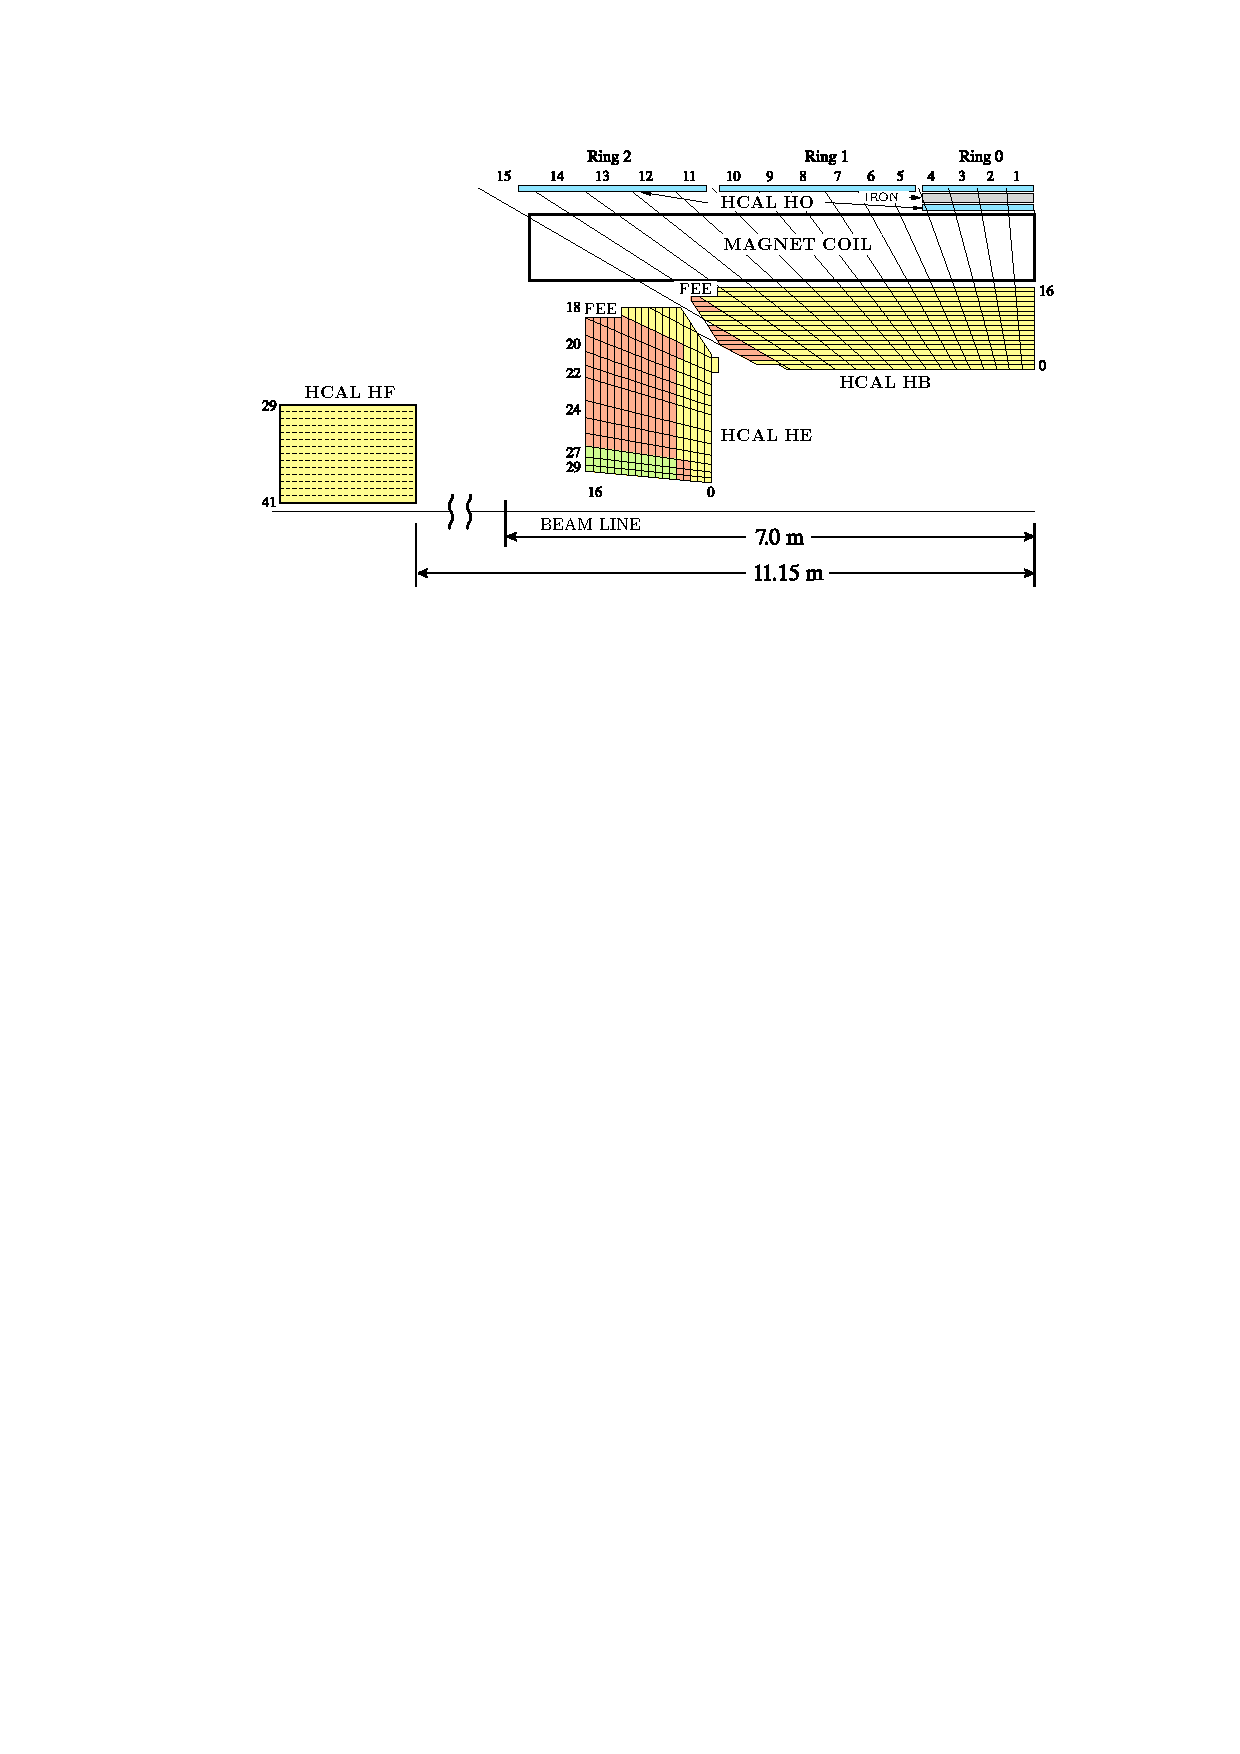
\includegraphics[width=.95\textwidth]{pics/hcal_diagram}
\end{center}
\caption{Kinematic acceptance of the CMS HCAL}
\label{fig:hcal_diagram}
\end{figure}

Surrounding the ECAL. The Hadronic Calorimeter (HCAL) is designed to measure the the energy of neutral hadrons which do not
deposit the majority of their energy in the ECAL. 

 The HCAL consists of four sections: the barrel (HB), the endcap (HE), two forward calorimeters (HF) and an outer  hadron calorimieter (HO). 
The barrel and endcap of the HCAL cover $|\eta| < 4$. The forward detectors extend the subdetector's reach to $|\eta| =5$. The Outer Calorimieter exists to contain extremely high energy jets from reaching the muon chambers. 
While electrons and photons deposit nearly all of their energy in the ECAL, high energy hadrons deposit most of their energy in the HCAL.

The detector is constructed as  alternating layers of brass absorber and plastic scintillator



\begin{figure}
\begin{center}
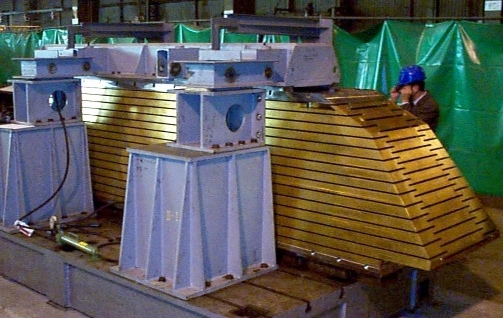
\includegraphics[width=.45\textwidth]{pics/hb_wedge}
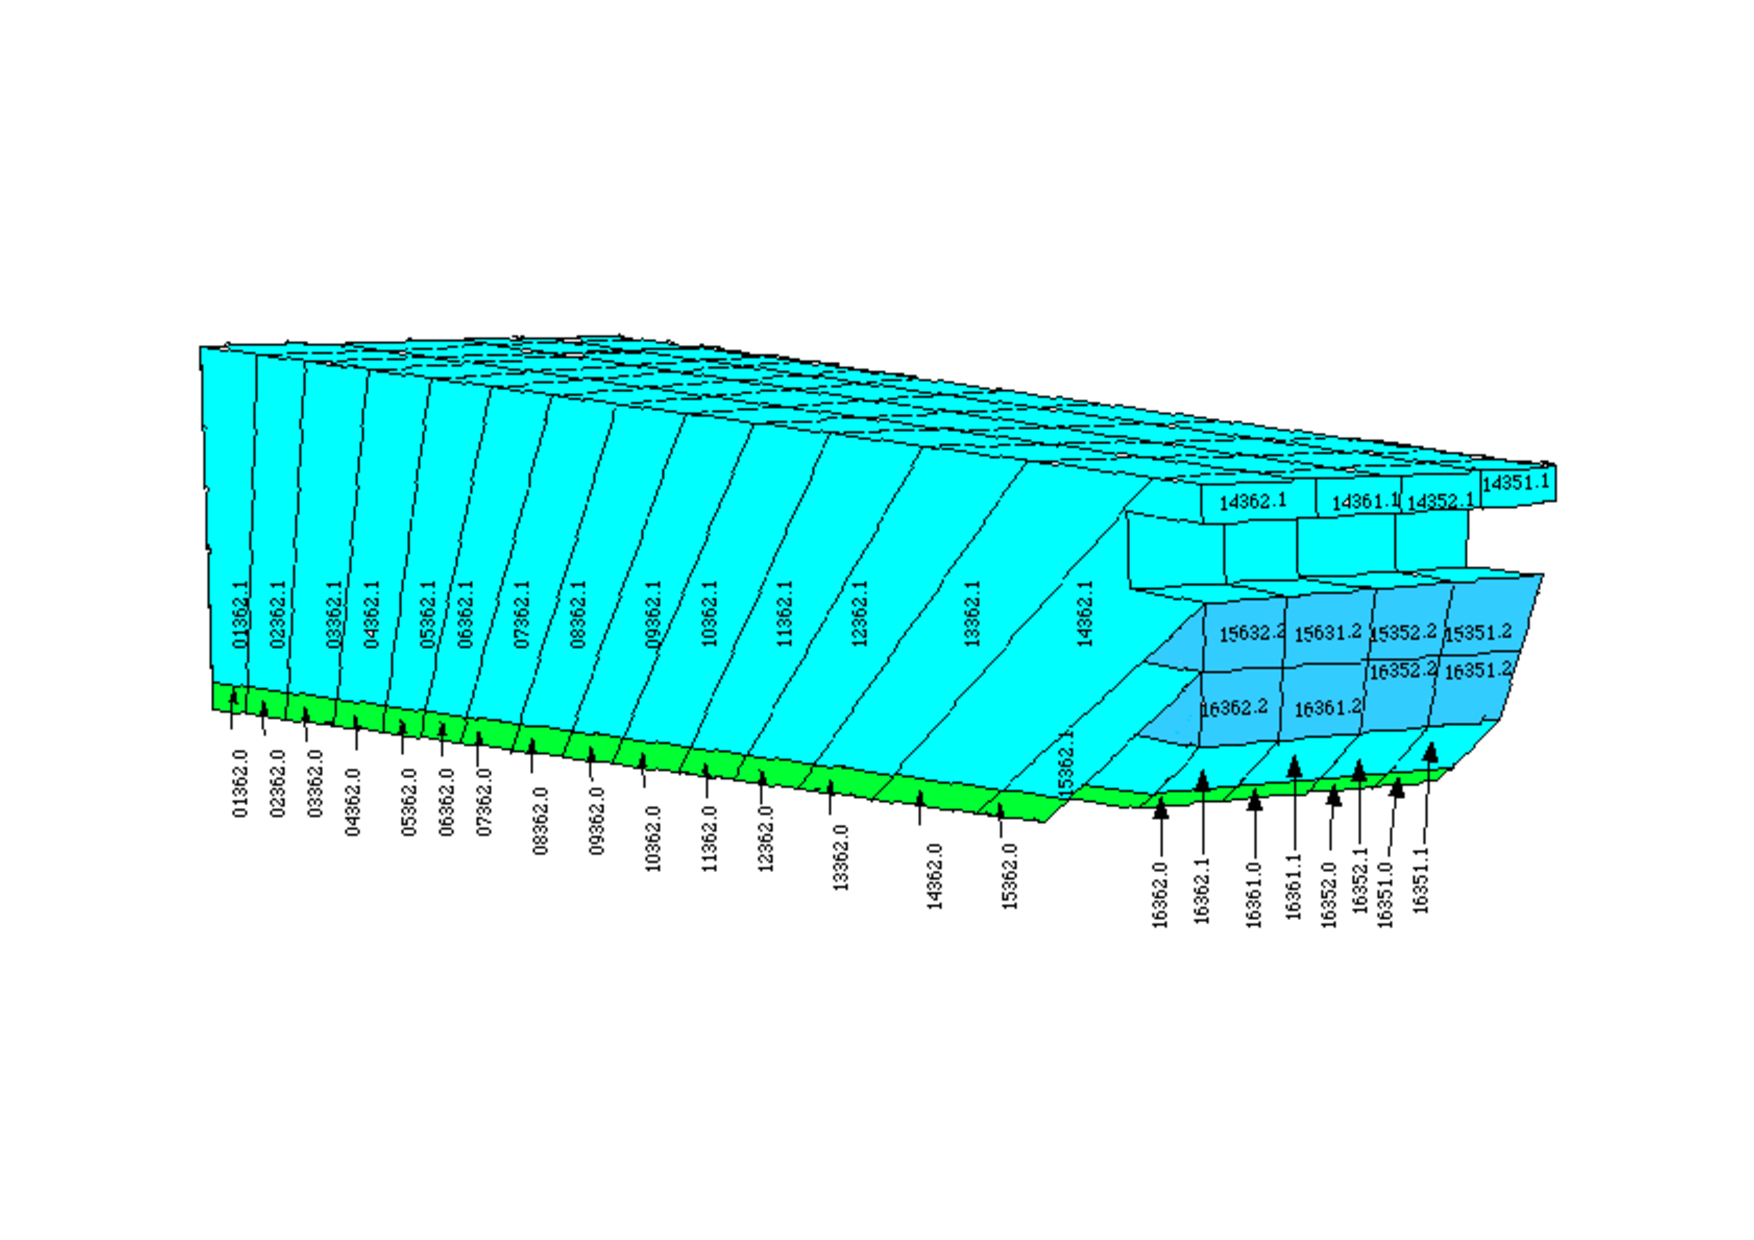
\includegraphics[width=.45\textwidth]{pics/hb_diagram}
\end{center}
\caption{A single wedge of the CMS HCAL barrel}
\label{fig:hb_wedge}
\end{figure}

\begin{figure}
\begin{center}
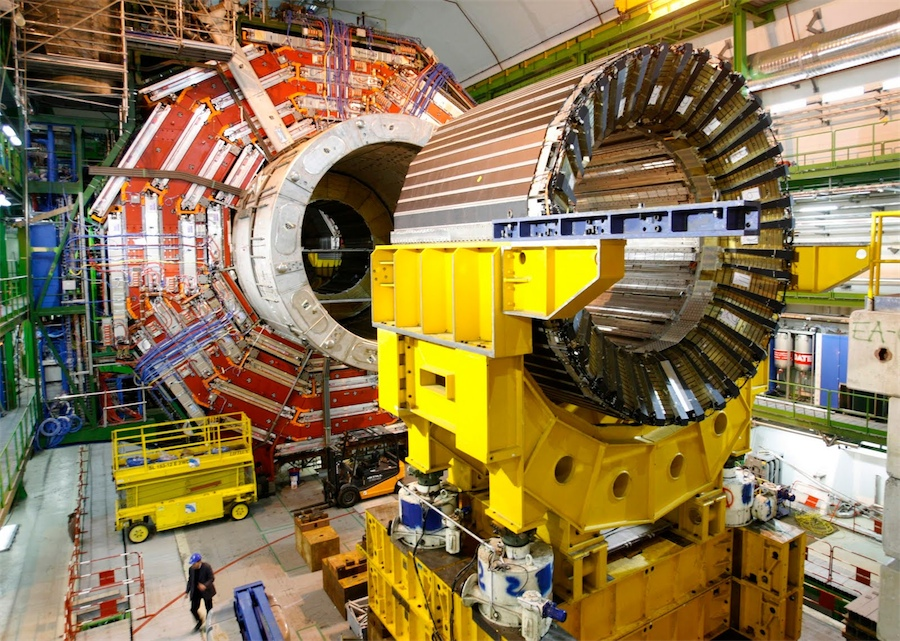
\includegraphics[width=.65\textwidth]{pics/naked_hcal}
\end{center}
\caption{The CMS HCAL outside of the detector}
\label{fig:hcal_naked}
\end{figure}

\subsection{Superconducting Solenoid}


\begin{figure}
\begin{center}
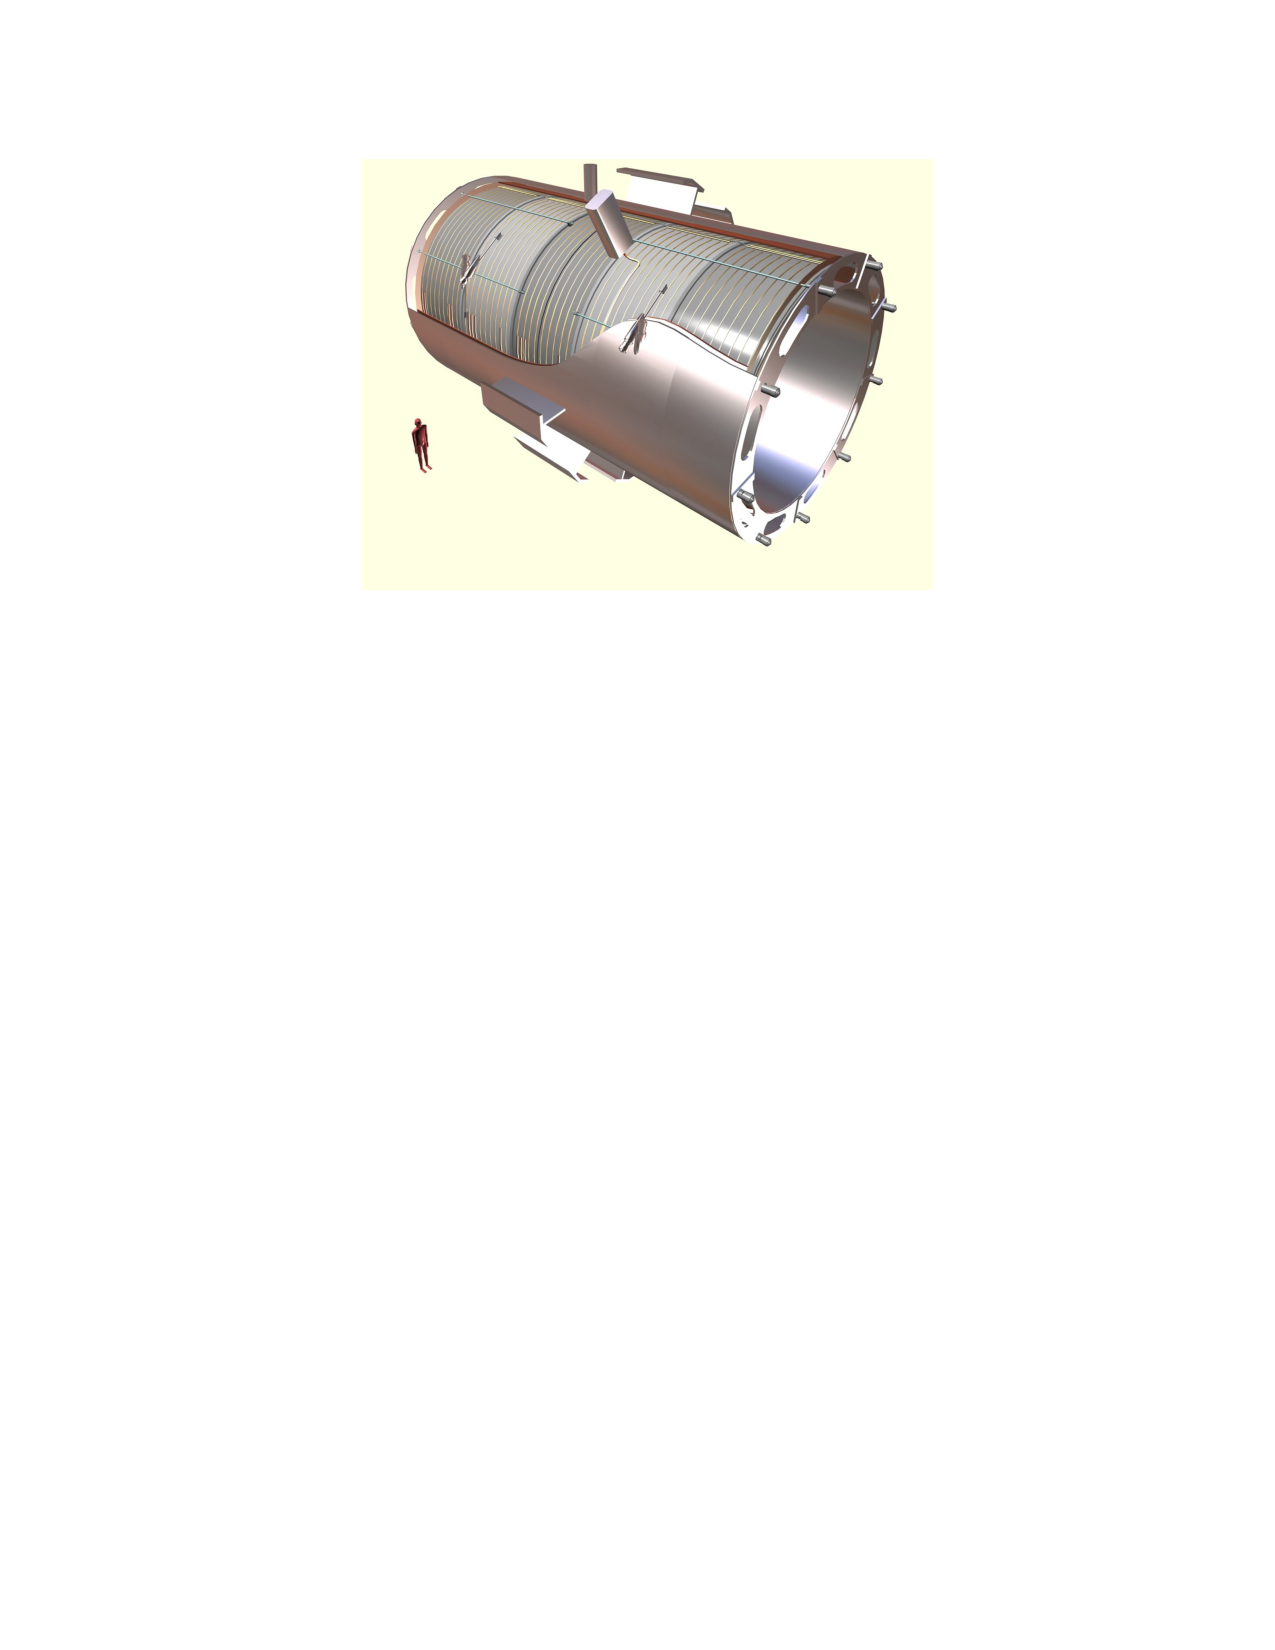
\includegraphics[width=.45\textwidth]{pics/solenoid_diagram}
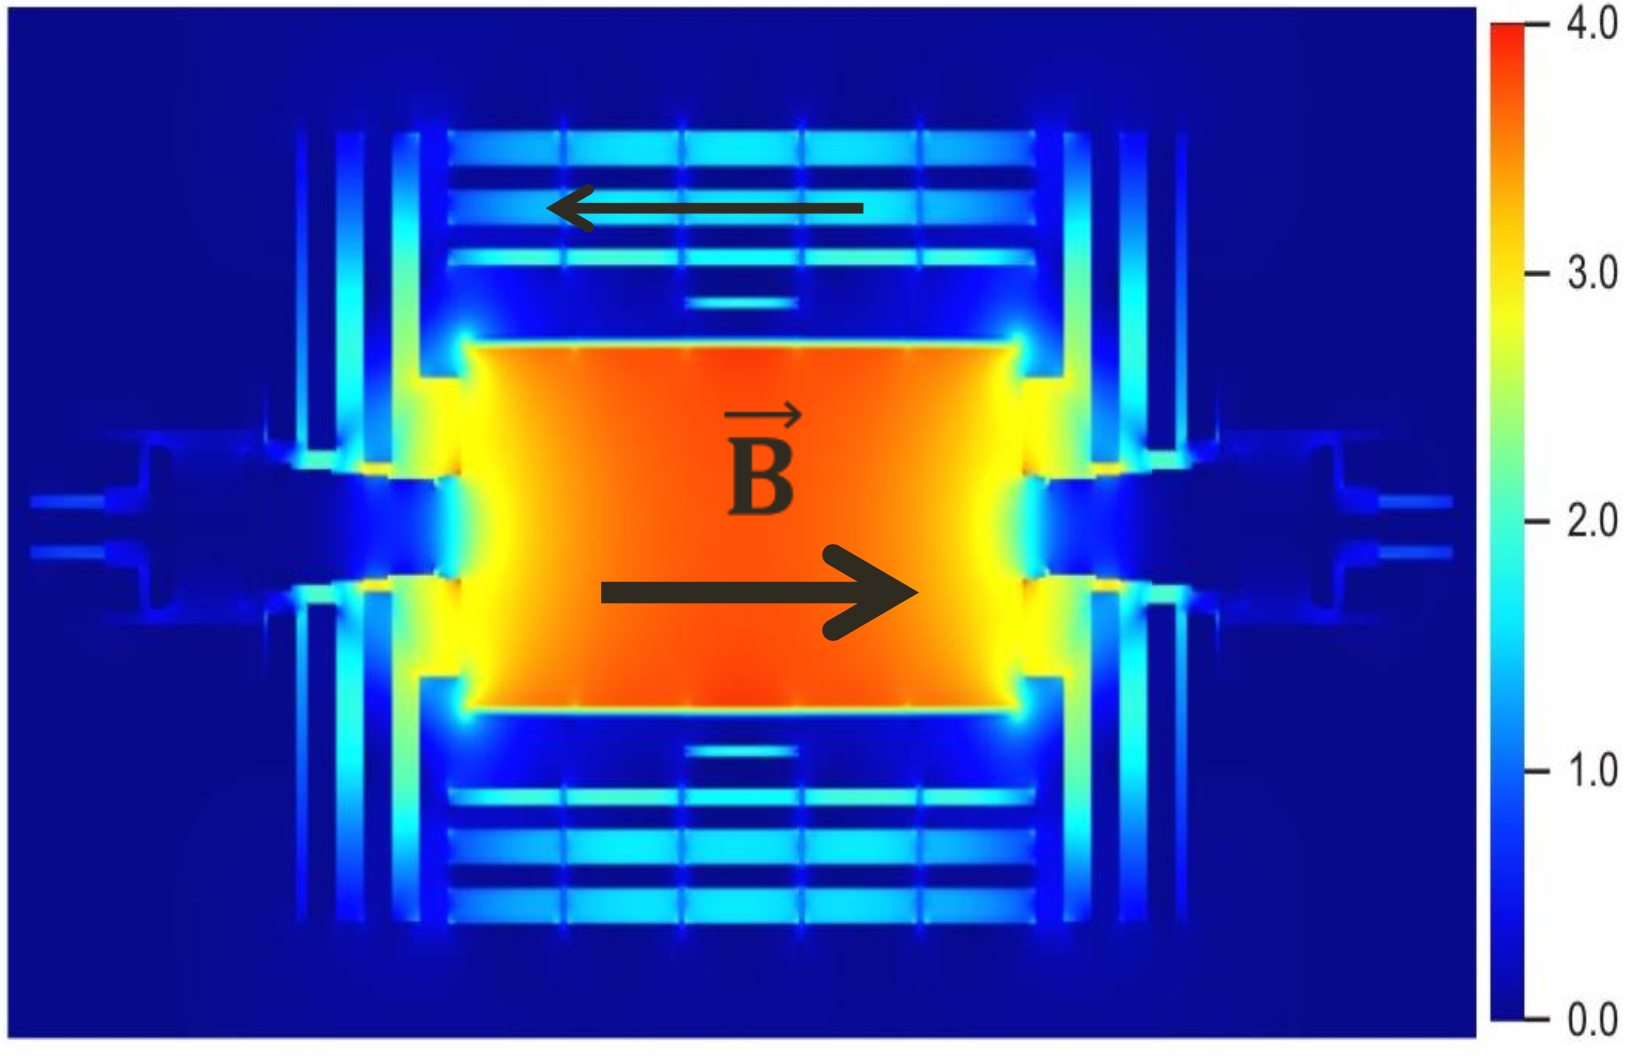
\includegraphics[width=.45\textwidth]{pics/b_field}
\end{center}
\caption{The CMS solenoid with a human for scale}
\label{fig:solenoid_bfield}
\end{figure}


\subsection{Tracking}

\begin{figure}
\begin{center}
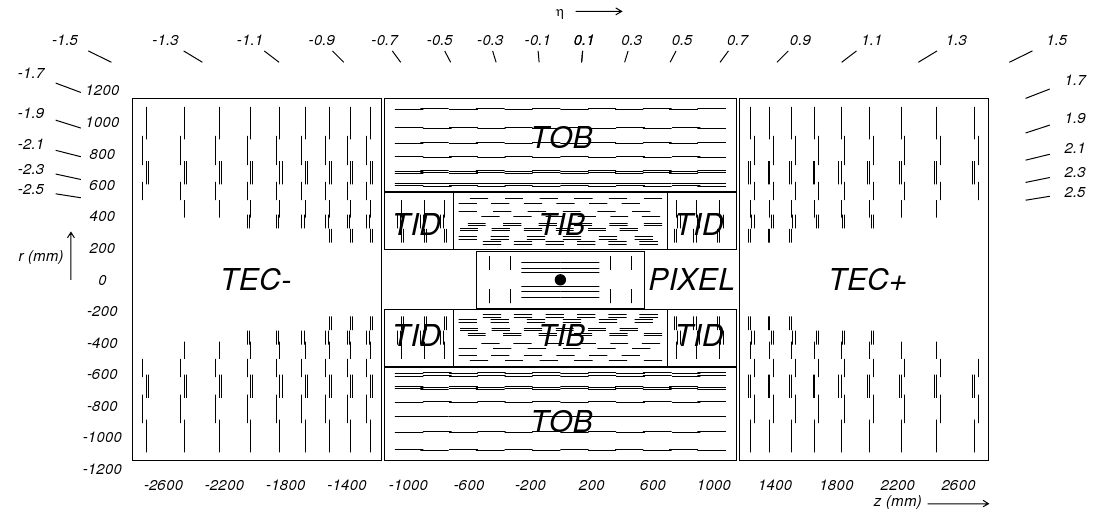
\includegraphics[width=.95\textwidth]{pics/tracker_diagram}
\end{center}
\caption{Kinematic acceptance of the CMS tracker}
\label{fig:tracker_diagram}
\end{figure}

\begin{figure}
\begin{center}
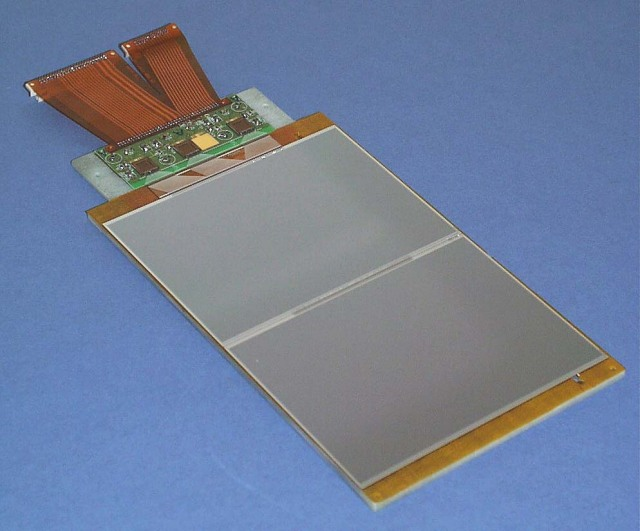
\includegraphics[width=.45\textwidth]{pics/tracker_module}
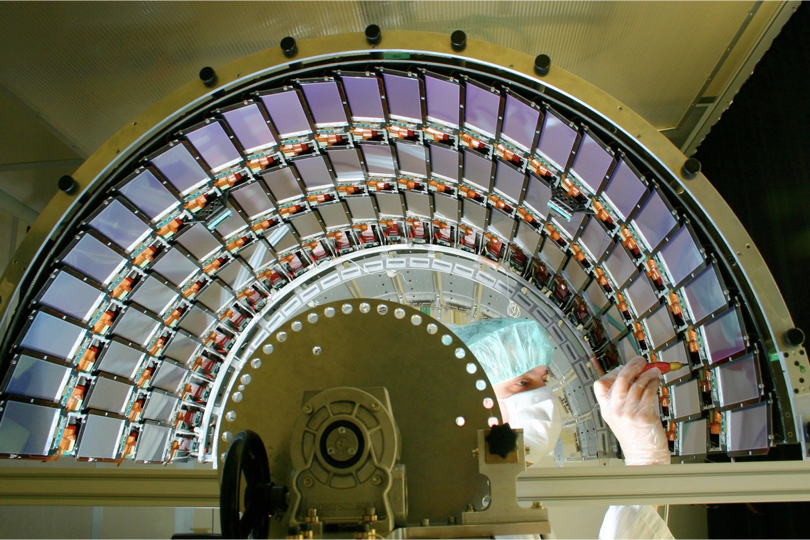
\includegraphics[width=.45\textwidth]{pics/tracker_strips}
\end{center}
\caption{A single CMS tracker module (left) and a tracker inner barrel module (right)}
\label{fig:tracker_strips_and_module}
\end{figure}

\begin{figure}
\begin{center}
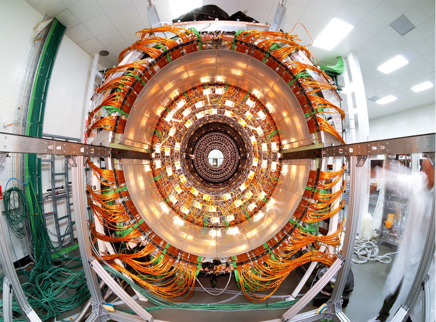
\includegraphics[width=.45\textwidth]{pics/naked_pixel}
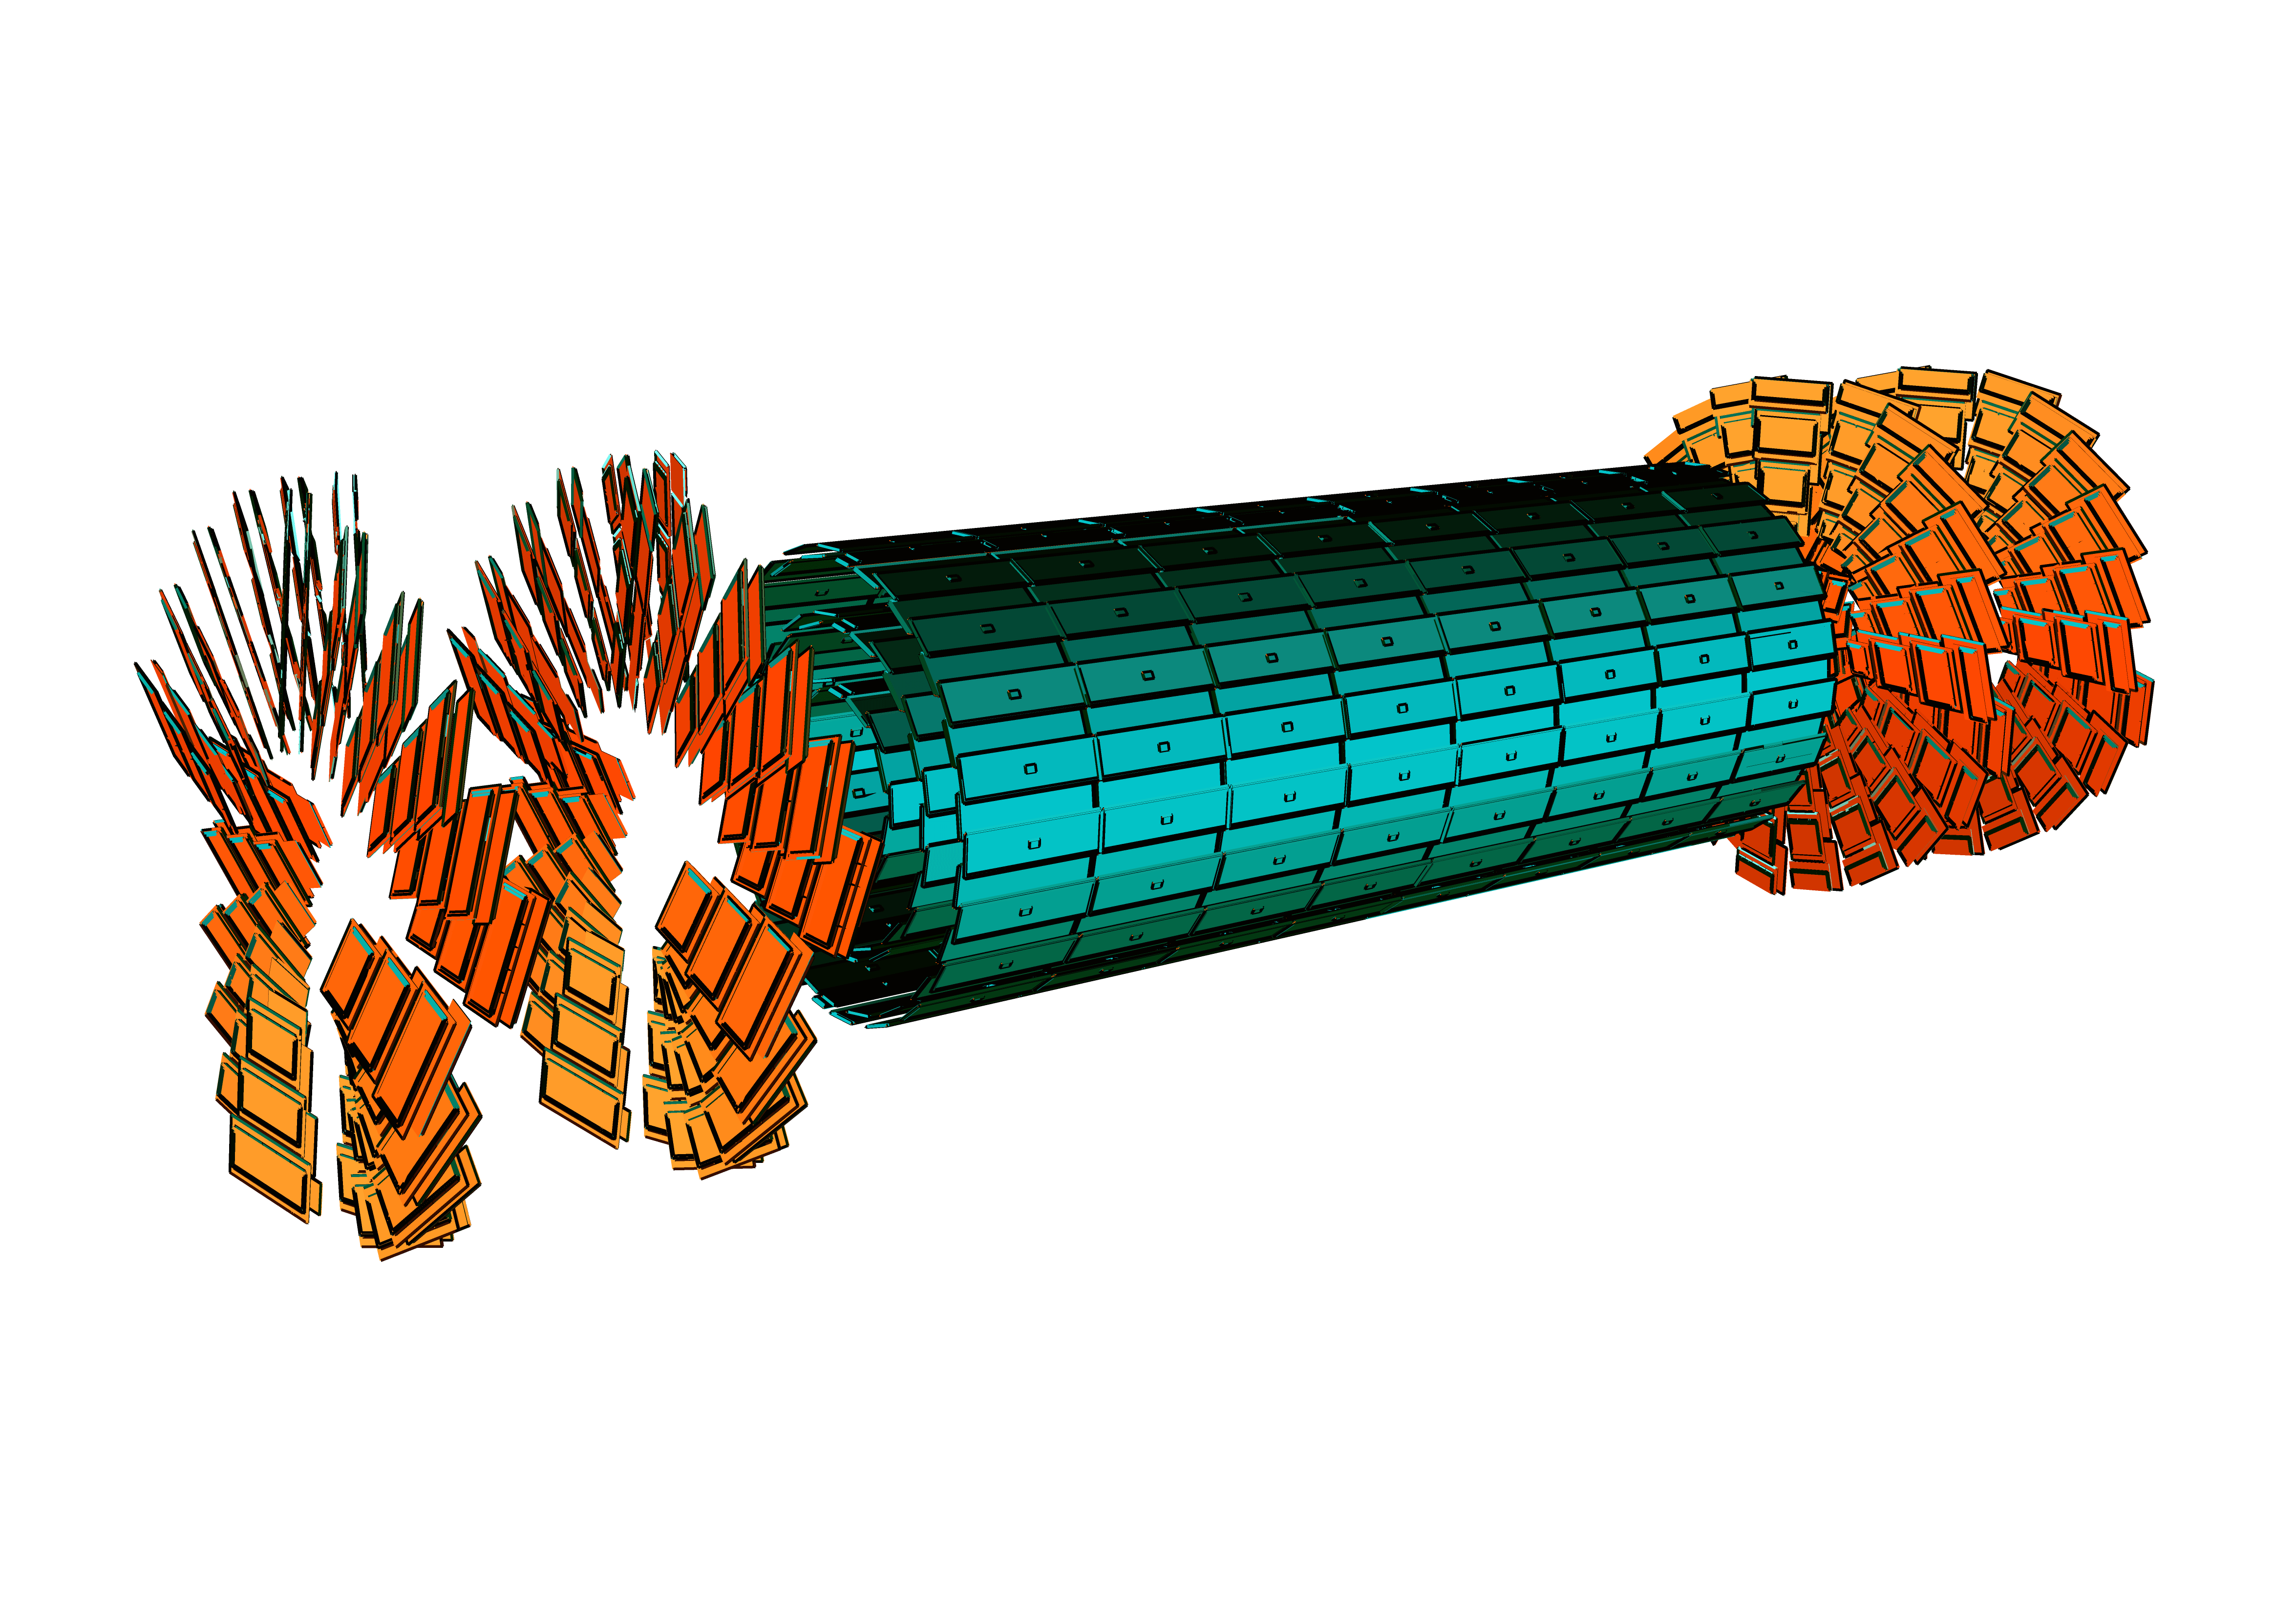
\includegraphics[width=.45\textwidth]{pics/pixel_diagram}
\end{center}
\caption{The CMS Pixel detector }
\label{fig:tracker_solenoid}
\end{figure}

\begin{figure}
\begin{center}
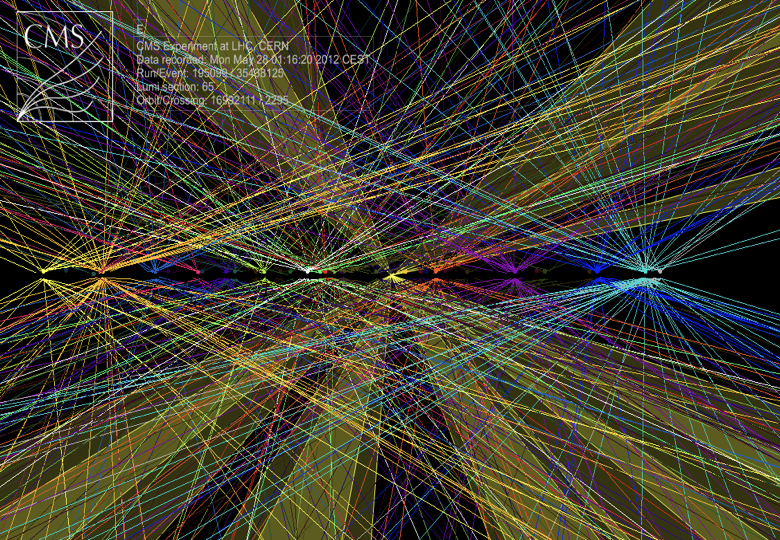
\includegraphics[width=.75\textwidth]{pics/pileup_vertices}
\end{center}
\caption{Pileup Interactions}
\label{fig:pileup}
\end{figure}

\subsection{Muon Chambers}

\begin{figure}
\begin{center}
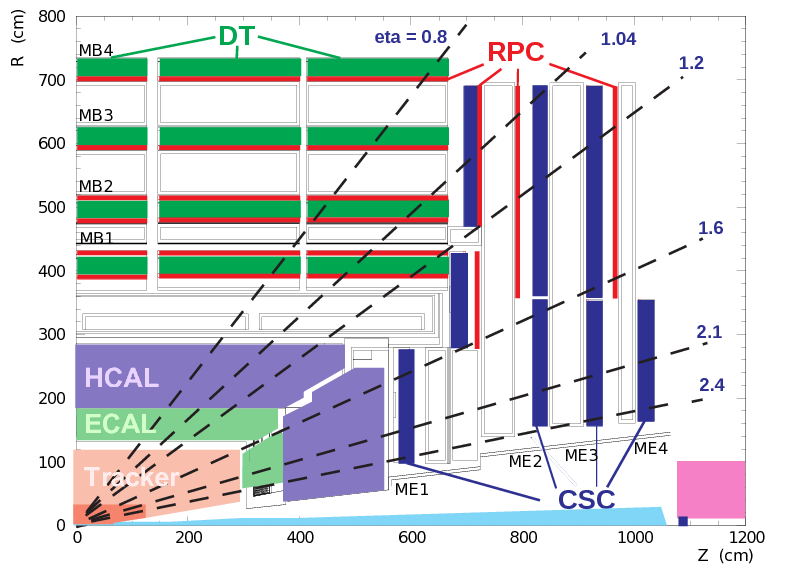
\includegraphics[width=.85\textwidth]{pics/muon_diagram}
\end{center}
\caption{Kinematic acceptance of the CMS Muon System}
\label{fig:muon_diagram}
\end{figure}

\begin{figure}
\begin{center}
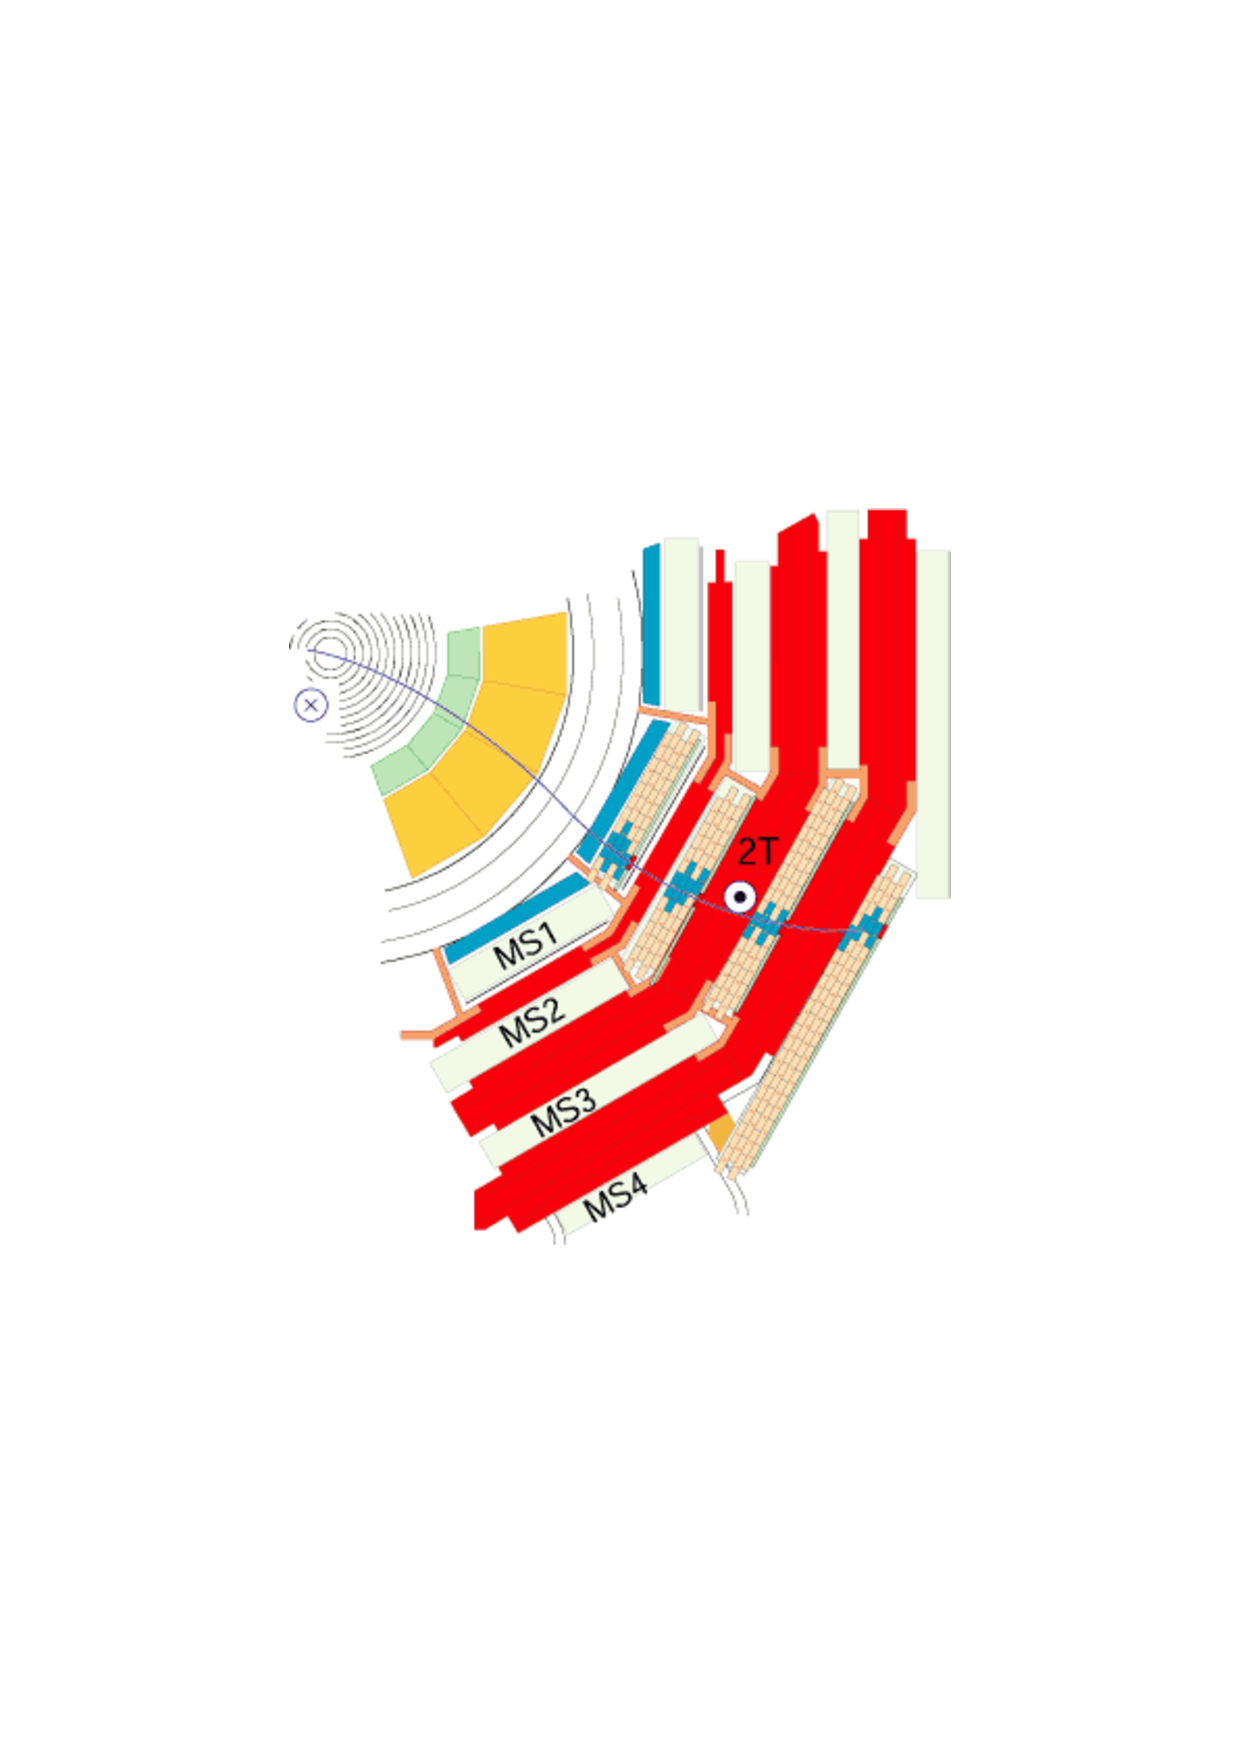
\includegraphics[width=.45\textwidth]{pics/muon_slice}
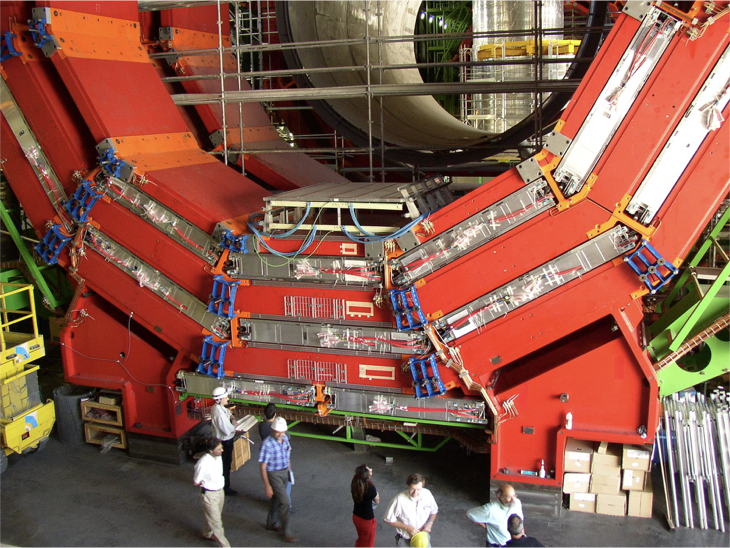
\includegraphics[width=.45\textwidth]{pics/rpc_plates}
\end{center}
\caption{The Muon RPC Plates}
\label{fig:muon_slice}
\end{figure}

\begin{figure}
\begin{center}
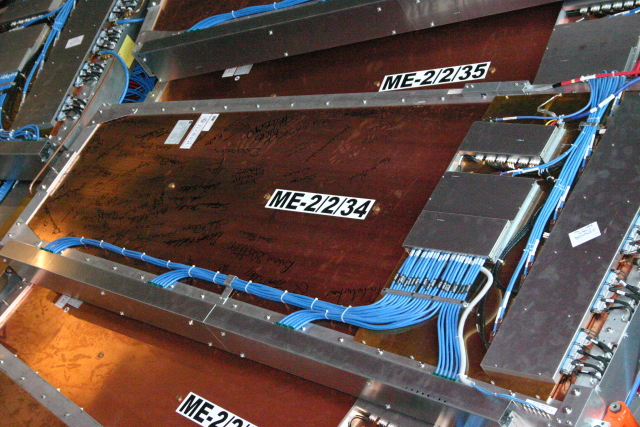
\includegraphics[width=.45\textwidth]{pics/cathode_strip_chamber}
\end{center}
\caption{The Muon Cathode Strip Chamber}
\label{fig:strip_chamber}
\end{figure}

\subsection{Trigger System}

\begin{figure}
\begin{center}
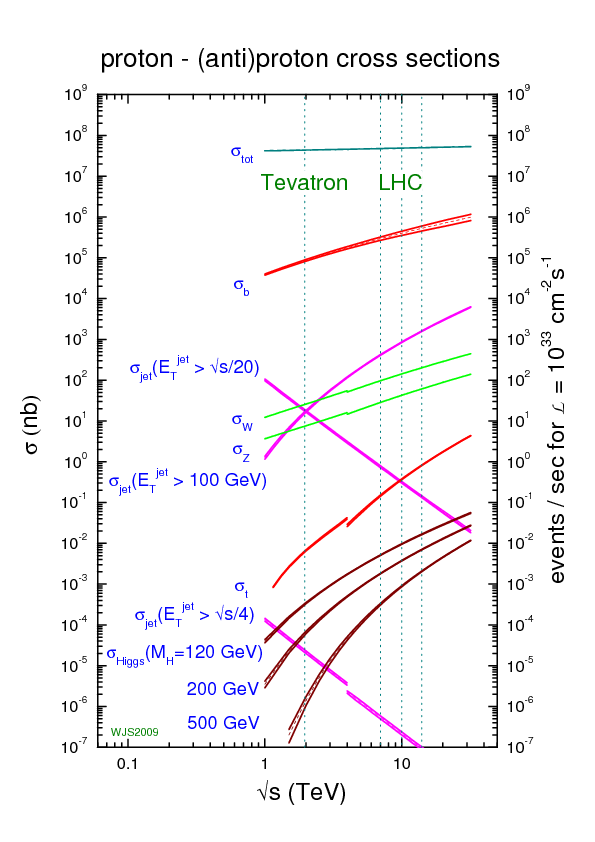
\includegraphics[width=2.9in]{figures/exp_proj/pdf_xsec.png}
\caption{Common cross sections of proton collisions as a function of the center of mass energy $\sqrt{s}$}
\end{center}
\label{fig:pdf_xsec}
\end{figure}

The CMS Trigger System exists as a filter through which events are determined to be ``interesting''. 
It is both  unnecessary and inefficient to record anything that occurs in the detector electronics. 
Most events that occur from colliding protons are well understood. To the left, you can see the 
logarithmic plot of common physics processes for proton-proton scattering. Events such as the production 
of a $b$ quark  occur at $\approx 10^6$ Hz at a luminosity of $\mathcal{L} = 10^{33}$ cm$^{-2}$ 
whereas the production of the Higgs is much lower at $\approx 10^{-2}$ Hz.  

At design luminosity, the LHC has beam crossings at a rate of $\approx 40$ MHz with 
each crossing coming spaced at $\approx$ 25 ns. 
For each crossing there are $\approx$ 20 inelastic collisions (referred to as pile up) 
contained in an event file of $\approx$ 1 Mb. 
However the bandwidth for storage is limited to $\approx 10^2$ Hz and equivalently $10^2$ Mb/s. 
Generally, all but one of the inelastic collisions is interesting and a large excess of uninteresting 
activity is generated in the detector electronics. The trigger must be robust enough to select 
this needle in a haystack event while remaining computationally efficient in maximizing the limited bandwidth.  

The CMS Trigger system is designed to read events at the event crossing frequency and generate the
 factor $10^5$ of rejection between the crossing frequency and the archival capacity. This factor 
is far too large to achieve in a single step given the complexity of triggers and event reconstruction. 
Therefore the task is split into two steps: The Level 1 (L1) and High Level (HLT) Trigger systems.

The $O(10^7$) events per second first pass through the L1 Trigger which reads out events at $10^5$ Hz. 
From here, the High Level Trigger makes the final decision as to which events are kept. 
Approximately 350 Hz is processed and stored, 300 Hz is ``parked'' (stored but processed later), 
and 1 kHz is partially stored (only the HLT level information and not the RAW detector information) 
and used for data scouting for future analysis.  

The most basic criterion for interesting events are hard physics events with high momentum transfer, $q^2$.
 As the protons collide with effectively no transverse momentum, any event with significant deposits of 
transverse energy (or even missing transverse momentum) is indicative of a hard physics process. 
The number of objects with a given transverse momentum falls off exponentially, so a simple minded way to
  reduce the rate of processed events is to raise the threshold of accepted events. 

More specific criterion for ``interesting events'' is analysis dependent. Generally, analyses are
 categorized by their final state signature. Thus, the trigger requires loose identification 
on the objects of that signature such as the isolation and shape of energy deposition. 
Once the event has passed the Level 1 and HLT Triggers, tighter and more computationally 
costly selection can be made offline where we are unrestricted by bandwidth limitations. 

As there is a limited amount of bandwidth for processing the events, the numerous analyses of CMS
 are given a budget (measured in Hz) for the triggers they request. As it stands the $H\rightarrow \gamma\gamma$ 
analysis is assigned a budget of 30 Hz for its diphoton trigger suite. As the diphoton channel was of 
high priority in the 7 and 8 TeV running this accounted for a significant fraction ($\approx$10\%) of the overall budget. 

As the luminosity of the machine increases, we expect proportionally more events per second and must accordingly alter the triggers. 

\begin{figure}
\begin{center}
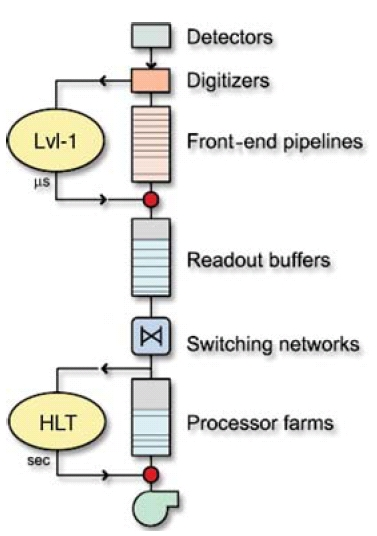
\includegraphics[width=2.5in]{figures/exp_proj/cms-trigger}\\
\caption{A diagrammatic representation of the level 1 and HLT trigger processing}
\end{center}
\end{figure}


\subsubsection{Level 1 (L1) Trigger}

\subsubsection{High Level Trigger (HLT)}

